\documentclass[10pt,a4paper]{article}
\usepackage[margin=25mm]{geometry}
\usepackage{amsmath,amssymb,amsthm,graphicx,hyperref}
\usepackage[dvipsnames]{xcolor}
\newcommand{\binampersand}{\mathbin{\&}}
\newcommand{\bindnasrepma}{\mathbin{\rotatebox[origin=c]{180}{\&}}}
\sloppy
\title{Proof-relevant Craig-Lyndon interpolation in first-order linear logic by cut introduction}
\author{Alexis Saurin}
\date{doi:10.4230/LIPIcs.FSCD.2025.32; CC BY4.0}
\begin{document}
\maketitle
\noindent\textit{Editorial note.} Only the general proof-relevant Craig-Lyndon interpolation Theorem5 is counted. Its equivalent restatement, LK/LJ consequences and individual proof-rule cases remain uncounted support. All AppendixA cases retained.\par\medskip
\noindent\textit{Editorial note.} Official CC BY4 publisher HTML retained. TeX is copied from original MathML alttext; seventy-seven original proof/inference SVG diagrams are rendered to vector PDF and preserved. No proof redrawing, mathematical paraphrase or supplied deductions.\par\medskip
\noindent\textit{Editorial scope.} Complete author material collection for one structural theorem; author retains responsibility for the mathematics.\par\medskip
\noindent\textit{Allowed standard prerequisites (editorial).}\begin{itemize}
\item First-order linear logic sequent calculus, cut reduction and polarized vocabulary. All exact author rules, ancestor relation and vocabulary conventions retained in Section2.
\item Maehara interpolation framework. Author precise proof-relevant refinement and all specialized PRIS/cut-expansion cases retained; no ordinary interpolation theorem substituted for the counted stronger reconstruction claim.
\end{itemize}\medskip

% BEGIN S1
 
\par\medskip\noindent\textbf{1 “– Why Not a Proof-Relevant Interpolation Theorem?  – Introduce Cuts, Of Course!”}\par
 
% BEGIN S1.p1
 
In the words of Solomon Feferman, “though deceptively simple and plausible on the face of it, Craig’s interpolation theorem (…) has proved to be a central logical property that has been used to reveal the deep harmony between the syntax and semantics of first order logic” [17]. Indeed, Craig’s interpolation (which states that in the predicate calculus, if $A\vdash B$, there exists a formula $C$ built from the relation symbols occurring both in $A$ and $B$ such that $A\vdash C$ and $C\vdash B$) and its developments suggest far deeper connections between models and proofs than the simple correspondence between provability and validity given by Gödel completeness theorem. This could be argued to be in line with and pursue structural proof-theoretic proofs of Gödel completeness theorem such as Schütte proof [35] or the more recent analysis by Basaldella and Terui of completeness in Ludics [3, 2].\par
 
% END S1.p1
 
% BEGIN S1.p2
 
First of all, one should recall that while the original proof of interpolation by Craig [7, 8] was proof-theoretic as well as Maehara’s method [25] its most striking applications were model-theoretic results whether we consider standard model-theoretic results that are consequences of interpolation, such as Beth definability theorem [4] or Robinson’s consistency theorem [33] or if we consider modern uses of interpolation in model-checking [21, 27]. Among the proof-theoretical methods for proving interpolation, the success of Maehara’s method is probably due to its wide applicability to a range of logics and proof-systems, from intuitionistic logic [28, 35] to modal logics [18, 24, 1, 36] or in infinitary logics and abstract model theory [17, 15].\par
 
% END S1.p2
 
% BEGIN S1.p3
 
While in most proof theory textbooks [20, 35, 39, 40] Craig’s interpolation theorem is presented as an application of cut-elimination, one shall see here that it also has in fact much to do with cut-introduction, giving a proof-relevant and computational content to Interpolation theorem. This opens the way to an analysis of interpolation in terms of the denotational semantics of proofs and programs.\par
 
% END S1.p3
 
% BEGIN S1.SS0.SSS0.P0.SPx1
 
\par\medskip\noindent\textbf{Contributions and organization of the paper.}\par
 
% BEGIN S1.SS0.SSS0.P0.SPx1.p1
 
More precisely, after providing background on linear logic sequent calculus in Section 2, we state in Section 3 the following result for first-order linear logic ($\mathsf{LL}$ in the following): For any first-order $\mathsf{LL}$ formulas $A,B$, if $\pi$ proves $A\vdash B$, there exists a formula $C$ in the common vocabulary (that refers to the subset of the first-order language occurring in a formula, in terms of relation symbols, possibly taking into account polarity constraints as in Lyndon’s interpolation) of $A$ and $B$ and proofs $\pi_{1},\pi_{2}$ of $A\vdash C$ and $C\vdash B$ respectively such that ${\text{\scriptsize$(\mathsf{Cut})$}}(\pi_{1},\pi_{2})$, that is $\pi_{1}$ composed with $\pi_{2}$, is equivalent to $\pi$ (by $=_{\mathsf{cut}}$ we refer to the congruence generated by the cut-reduction rules):\par
 
% END S1.SS0.SSS0.P0.SPx1.p1
 
% BEGIN S1.SS0.SSS0.P0.SPx1.p2
 
\begin{center}
\includegraphics[width=0.95\linewidth,height=0.45\textheight,keepaspectratio]{graphic-01.pdf}\end{center}
 
% END S1.SS0.SSS0.P0.SPx1.p2
 
% BEGIN S1.SS0.SSS0.P0.SPx1.p3
 
Interpolation can therefore be achieved while preserving the computational / denotational content of proofs, while factoring the computation through an interfacing, interpolant type made only of the base types used in both the input and output types.\par
 
% END S1.SS0.SSS0.P0.SPx1.p3
 
% BEGIN S1.SS0.SSS0.P0.SPx1.p4
 
This result is then extended to classical and intuitionistic logics simply by means of linear translations, which sheds an interesting light on the relationship between Lyndon and Craig’s interpolation.\par
 
% END S1.SS0.SSS0.P0.SPx1.p4
 
% BEGIN S1.SS0.SSS0.P0.SPx1.p5
 
Then, by a further analysis of Maehara’s method, we show in Section 4 that the interpolation process for a cut-free proof deriving $A\vdash B$ can be in fact decomposed in two phases: (i) an ascending phase which equips each sequent of $\pi$ with a splitting is followed by (ii) a descending phase which solves the interpolation problem. This latter descending phase happens to be a cut-introduction phase which provides a proof of the proof-relevant interpolation result of the previous section. In particular, the resulting proof is, by construction, denotationally equal to $\pi$.\par
 
% END S1.SS0.SSS0.P0.SPx1.p5
 
% BEGIN S1.SS0.SSS0.P0.SPx1.p6
 
Finally, in Section 5, we consider the computational content of interpolation and address this question using the framework of the Duality of Computation introduced by Curien and Herbelin: we consider the linear system L, a term calculus with typing rules very close to that of the sequent calculus111System L can be viewed as achieving a Curry-Howard correspondence with sequent calculus proofs – while the $\lambda$-calculus achieves a correspondence with natural deduction proofs, and prove a computational interpolation result.\par
 
% END S1.SS0.SSS0.P0.SPx1.p6
 
% END S1.SS0.SSS0.P0.SPx1
 
% BEGIN S1.SS0.SSS0.P0.SPx2
 
\par\medskip\noindent\textbf{Related works.}\par
 
% BEGIN S1.SS0.SSS0.P0.SPx2.p1
 
Surprisingly we could not find any occurrence in the literature analyzing Maehara’s method in terms of cut-elimination (or rather, cut-introduction) even though all ingredients were there since Maehara’s seminal work.\par
 
% END S1.SS0.SSS0.P0.SPx2.p1
 
% BEGIN S1.SS0.SSS0.P0.SPx2.p2
 
On the other hand, another early proof-theoretic proof of interpolation theorem was proposed by Prawitz for natural deduction [31]. Just like for Maehara’s method the strengthened, proof-relevant interpolation result was at hand in this work as well and Čubrić actually showed this in the setting of the simply typed $\lambda$-calculus as well as a corresponding factorization result for bicartesian closed categories in the early 90s [9, 10]. Sadly, Čubrić’s paper as well as his PhD thesis supervised by Makkai, received too little attention and very few following works refer to his results: we could only find less than 10 references to these works among them only three truly consider the interpolation aspect [16, 26, 23]222Matthes [26] extends Čubrić’ results to a natural deduction with general elimination rules and a corresponding term calculus while Kanazawa [23] considers interpolation in purely implicational fragments of intuitionistic logic and finds workarounds for the lack of interpolation in this setting. On the way, he considers various sequent calculi and proves a result which has some similarities with our result but is weaker both in terms of the logical language – which is restricted to implicative $\mathsf{LJ}$– and of the characterization of the equivalence between the interpolating proofs and the original proof.. We hope that the present work can contribute to foster interest in Čubrić results.\par
 
% END S1.SS0.SSS0.P0.SPx2.p2
 
% BEGIN S1.SS0.SSS0.P0.SPx2.p3
 
Another related work is that of Carbone [6] where she establishes a strengthened form of Maehara’s interpolation paying great attention to the ancestor relation (formulated in terms of flow graphs in that work) which allows her to get bounds on the complexity of the interpolant but did not lead her to a study of proof-relevant interpolation, invariance by cut-elimination nor interpolation as cut-introduction. Only few works consider interpolation in (fragments of) linear logic, starting with Roorda [34]. In the framework of the calculus of structure, Straßburger proves a decomposition theorem for $\mathsf{MELL}$ [37] that is advocated to correspond to an interpolation theorem and may have a more fine-grained proof-theoretical content. More recently, several papers investigated and formalized interpolation theorems in substructural logics, including exponential-free linear logic [5, 14, 32].\par
 
% END S1.SS0.SSS0.P0.SPx2.p3
 
% END S1.SS0.SSS0.P0.SPx2
 
% END S1


% BEGIN S2
 
\par\medskip\noindent\textbf{2 Background on LL proof theory}\par
 
% BEGIN S2.p1
 
In the following, we provide the necessary background on first-order $\mathsf{LL}$.\par
 
% END S2.p1
 
% BEGIN S2.p2
 
As usual, we assume a first-order language $\mathcal{L}$ (without equality nor function symbols). We assume the set of atomic formulas to be equipped with an involution, inducing a partitioning between positive atomic formulas, written $a$, and negative atomic formulas, written $a^{\perp}$. We introduce a language of first-order $\mathsf{LL}$ formulas:\par
 
% END S2.p2
 
% BEGIN Thmtheorem1
 
\par\medskip\noindent\textbf{Definition 1.}\par
 
% BEGIN Thmtheorem1.p1
 
The grammar of first-order $\mathsf{LL}$ formulas is defined inductively as:\par
    \[\begin{array}[]{lrlllllr}F&::=&a^{\perp}&\mid\leavevmode\nobreak\ \perp\leavevmode\nobreak\ \leavevmode\nobreak\ \leavevmode\nobreak\ \mid\leavevmode\nobreak\ \top&\mid F\bindnasrepma F&\mid F\binampersand F&\mid\forall x.F&\textbf{negative \boldmath$\mathsf{MALL}$ formulas}\\
&\mid&a&\mid\leavevmode\nobreak\ 1\leavevmode\nobreak\ \leavevmode\nobreak\ \mid\leavevmode\nobreak\ 0&\mid F\hskip-1.0pt\otimes\hskip-1.0ptF&\mid F\oplus
F&\mid\exists x.F&\textbf{positive \boldmath$\mathsf{MALL}$ formulas}\\
&\mid&\mathop{?}F&\mid\mathop{!}F&&&&\textbf{exponential formulas}\end{array}\]    
% END Thmtheorem1.p1
 
% BEGIN Thmtheorem1.p2
 
Linear negation is defined as usual as an involution on $\mathsf{LL}$ formulas (changing $a^{\perp}$, $\bot$, $\top$, $\bindnasrepma$, $\binampersand$, $\forall$, $\mathop{?}$ into $a$, $1$, $0$, $\hskip-1.0pt\otimes\hskip-1.0pt$, $\oplus$, $\exists$, $\mathop{!}$ respectively). A one-sided $\mathsf{LL}$ sequent is an ordered list of $\mathsf{LL}$ formulas usually written $\vdash\Gamma$ to emphasize the sequent judgments.\par
 
% END Thmtheorem1.p2
 
% END Thmtheorem1
 
% BEGIN Thmtheorem2
 
\par\medskip\noindent\textbf{Definition 2 ($\mathsf{LL}$ sequent calculus).}\par
 
% BEGIN Thmtheorem2.p1
 
The inference rules of $\mathsf{LL}$ sequent calculus are given in Figure 1. The inferences of Figure 1 show a relation between conclusion and premises formulas, the ancestor relation (or sub-occurrence relation) that is extended by transitivity to formulas of non consecutive sequents of a derivation. An $\mathsf{LL}$ proof of a sequent $\vdash\Gamma$ is a finite tree rooted in $\vdash\Gamma$ generated by the rules of Figure 1.\par
 
% END Thmtheorem2.p1
 
% END Thmtheorem2
 
% BEGIN Thmtheorem3
 
\par\medskip\noindent\textbf{$\blacktriangleright$ Remark 3.}\par
 
% BEGIN Thmtheorem3.p1
 
The ancestor relation defined above is (implicitly) used in designing a cut-reduction system and plays a crucial role in expressing the validity condition for non-wellfounded and circular proofs as well as in the extension of Maehara’s method we will show next, in order to propagate sequent splittings from conclusions to premises.\par
 
% END Thmtheorem3.p1
 
% END Thmtheorem3
 
% BEGIN S2.F1

\begin{center}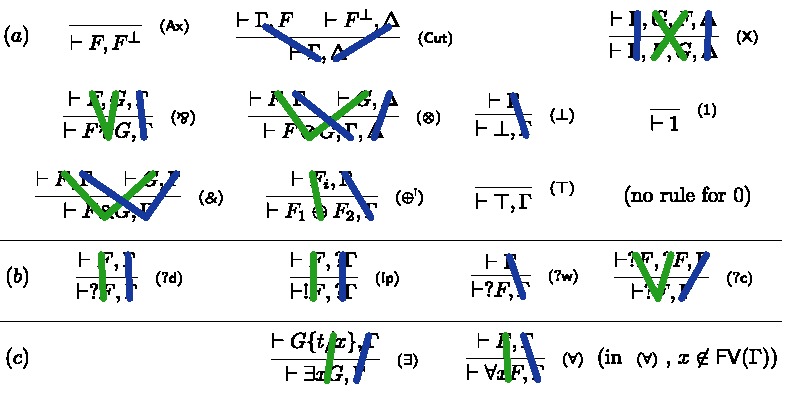
\includegraphics[width=0.95\linewidth,height=0.45\textheight,keepaspectratio]{graphic-02.pdf}\end{center}
 
Figure 1: (a) Propositional $\mathsf{MALL}$ Inferences; (b) $\mathsf{LL}$ Exponential Inferences; (c) First-order Inferences.\par
 
% END S2.F1
 
% BEGIN S2.p3
 
To state Craig-Lyndon interpolation, we need to make clear the required notion to express the interpolation condition on the vocabulary:\par
 
% END S2.p3
 
% BEGIN Thmtheorem4
 
\par\medskip\noindent\textbf{Definition 4 ((polarized) vocabulary of a formula).}\par
 
% BEGIN Thmtheorem4.p1
 
Given an $\mathsf{LL}$ formula $F$, $\mathbb{V}\mathsf{oc}(F)$ is the set of all predicate symbols occurring in $F$ together with their linear negations, while $\mathbb{V}\mathsf{oc}^{+}(F)$ (resp. $\mathbb{V}\mathsf{oc}^{-}(F)$) is the set of positive (resp. negative) predicate symbols occurring in $F$. This is naturally lifted to lists of formulas.\par
 
% END Thmtheorem4.p1
 
% END Thmtheorem4
 
% BEGIN S2.p4
 
In the present paper, we shall heavily rely on $\mathsf{LL}$ cut-reduction rules (and their symmetric, cut-introduction rules). The cut-reduction relation (resp. its reflexive and transitive and its reflexive, transitive and symmetric closures) is generically written $\longrightarrow_{\mathsf{cut}}$ (resp. $\longrightarrow^{\star}_{\mathsf{cut}}$ and $=_{\mathsf{cut}}$).\par
 
% END S2.p4
 
% END S2


% BEGIN S3
 
\par\medskip\noindent\textbf{3 Proof-relevant interpolation theorem}\par
 
% BEGIN S3.p1
 
The following proof-relevant interpolation theorem can be established by refining Maehara’s proof in order to take seriously into account the relations, not only between the interpolation sequents, but also between the interpolating proofs.\par
 
% END S3.p1
 

% BEGIN Thmtheorem5
 
\par\medskip\noindent\textbf{Theorem 5.}\par
 
% BEGIN Thmtheorem5.p1
 
Let $\Gamma,\Delta$ be lists of $\mathsf{LL}$ formulas and $\pi\vdash\Gamma,\Delta$ cut-free. There exists a $\mathsf{LL}$ formula $C$ such that $\mathbb{V}\mathsf{oc}^{+}{(C)}\subseteq\mathbb{V}\mathsf{oc}^{-}{(\Gamma)}\cap\mathbb{V}\mathsf{oc}^{+}{(\Delta)}$ and $\mathbb{V}\mathsf{oc}^{-}{(C)}\subseteq\mathbb{V}\mathsf{oc}^{+}{(\Gamma)}\cap\mathbb{V}\mathsf{oc}^{-}{(\Delta)}$ and two cut-free proofs $\pi_{1},\pi_{2}$ of $\vdash\Gamma,C$ and $\vdash C^{\perp},\Delta$ respectively such that\par
 
% END Thmtheorem5.p1
 
% BEGIN Thmtheorem5.p2
 
\begin{center}
\includegraphics[width=0.95\linewidth,height=0.45\textheight,keepaspectratio]{graphic-03.pdf}\end{center}
 
% END Thmtheorem5.p2
 
% END Thmtheorem5

 
% BEGIN S3.p2
 
In the following sections, we will follow two approaches which we consider to be more instructive from the computer science logic viewpoint, as they reveal the computational content of proof-relevant interpolation. We will proceed by “introducing cuts” so that we preserve the denotational equivalence of the interpolated proof with its interpolation (proofs).\par
 
% END S3.p2
 
% BEGIN S3.p3
 
But first, let us extend the proof-relevant interpolation result to $\mathsf{LK}$ and $\mathsf{LJ}$. These results could be obtained directly, by refining Maehara’s method or by following the cut-introduction or computational approach of the following section. On the other hand, one can directly deduce this result by using the linear embeddings of $\mathsf{LK}$ and $\mathsf{LJ}$ [19, 13] as a corollary of the above theorem.\par
 
% END S3.p3
 
% BEGIN Thmtheorem6
 
\par\medskip\noindent\textbf{Corollary 6.}\par
 
% BEGIN Thmtheorem6.p1
 
Let $\Gamma,\Gamma^{\prime},\Delta,\Delta^{\prime}$ be lists of $\mathsf{LK}$ formulas (resp. of $\mathsf{LJ}$ formulas, with $\Delta$ being empty and $\Delta^{\prime}$ of length at most 1) and $\pi$ be a cut-free $\mathsf{LK}$ (resp. $\mathsf{LJ}$) proof of $\Gamma,\Gamma^{\prime}\vdash\Delta,\Delta^{\prime}$.\par
 
% END Thmtheorem6.p1
 
% BEGIN Thmtheorem6.p2
 
There exists a $\mathsf{LK}$ (resp. $\mathsf{LJ}$) formula $C$ such that $\mathbb{V}\mathsf{oc}^{+}{(C)}\subseteq\mathbb{V}\mathsf{oc}^{+}{(\Gamma,\Delta)}\cap\mathbb{V}\mathsf{oc}^{+}{(\Gamma^{\prime},\Delta^{\prime})}$ and $\mathbb{V}\mathsf{oc}^{-}{(C)}\subseteq\mathbb{V}\mathsf{oc}^{-}{(\Gamma,\Delta)}\cap\mathbb{V}\mathsf{oc}^{-}{(\Gamma^{\prime},\Delta^{\prime})}$ and two cut-free $\mathsf{LK}$ (resp. $\mathsf{LJ}$) proofs $\pi_{1},\pi_{2}$ of $\Gamma\vdash C,\Delta$ and $\Gamma^{\prime},C\vdash\Delta^{\prime}$ respectively such that 
\begin{center}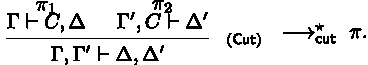
\includegraphics[width=0.95\linewidth,height=0.45\textheight,keepaspectratio]{graphic-04.pdf}\end{center}\par
 
% END Thmtheorem6.p2
 
% END Thmtheorem6
 
% BEGIN S3.SS0.SSS0.P0.SPx1
 
\par\medskip\noindent\textbf{Proof.}\par
 
% BEGIN S3.SS0.SSS0.P0.SPx1.p1
 
We sketch this here in the case of $\mathsf{LK}$.\par
 
% END S3.SS0.SSS0.P0.SPx1.p1
 
% BEGIN S3.SS0.SSS0.P0.SPx1.p2
 
First, it is a matter of a simple check that proof-relevant interpolation presented in the above theorem also holds for the two-sided $\mathsf{LL}$ sequent calculus.\par
 
% END S3.SS0.SSS0.P0.SPx1.p2
 
% BEGIN S3.SS0.SSS0.P0.SPx1.p3
 
Second, a cut-free $\mathsf{LK}$ proof $\pi$ (it would be similar for $\mathsf{LJ}$) can be decorated with exponential modalities and inferences in order to turn it into a cut-free $\mathsf{LL}$ proof $\pi^{\prime}$.\par
 
% END S3.SS0.SSS0.P0.SPx1.p3
 
% BEGIN S3.SS0.SSS0.P0.SPx1.p4
 
After interpolating this proof (obtaining $I^{\prime}$, $\pi^{\prime}_{1}$ and $\pi^{\prime}_{2}$), one can erase the linear information of the interpolants and the two interpolating proofs (that is, taking the classical skeleton of the proofs) and get back a pair of $\mathsf{LK}$ (resp. $\mathsf{LJ}$) proofs $\pi_{1},\pi_{2}$ together with a formula $I$ in $\mathsf{LK}$ (resp. $\mathsf{LJ}$) that lives in the appropriate vocabulary.\par
 
% END S3.SS0.SSS0.P0.SPx1.p4
 
% BEGIN S3.SS0.SSS0.P0.SPx1.p5
 
The properties of the linear embeddings ensure that the skeleton of a cut-free proof obtained from $\mathsf{Cut}(\pi^{\prime}_{1},\pi^{\prime}_{2})$ can be obtained by eliminating cuts from $\mathsf{Cut}(\pi_{1},\pi_{2})$. $\hfill\blacktriangleleft$\par
 
% END S3.SS0.SSS0.P0.SPx1.p5
 
% END S3.SS0.SSS0.P0.SPx1
 
% END S3



% BEGIN S4
 
\par\medskip\noindent\textbf{4 Interpolation as cut-introduction}\par
 
% BEGIN S4.p1
 
We will now show how the proof-relevant interpolation theorem stated in the previous section can be established by exploiting the dynamics of cut-introduction that is, more precisely, how the synthesis of the interpolant is in fact a cut-introduction process.\par
 
% END S4.p1
 
% BEGIN S4.p2
 
For this, we need to analyze and refine Maehara’s proof method.\par
 
% END S4.p2
 
% BEGIN S4.SS1
 
\par\medskip\noindent\textbf{4.1 Refining Maehara’s method}\par
 
% BEGIN S4.SS1.p1
 
The usual statement and proof method for interpolation, made more informative in the previous section, actually obfuscate the fact that the interpolating formula and proofs are synthetized using a cut-introduction mechanism: this is due to the structure of the inductive reasoning used to establish the interpolation theorem under Maehara’s method. Indeed, the inductive structure of the reasoning amounts to inspecting the structure of the sequent proofs until one reaches the base cases (the axiom and unit cases), after which the call to the induction hypotheses synthetize the interpolant.\par
 
% END S4.SS1.p1
 
% BEGIN S4.SS1.p2
 
Analyzing what happens in constructing the interpolating formula and proofs, for a cut-free proof $\pi$, is made clearer by structuring the process in two phases, a bottom-up phase and a top-down phase:\par
  Ascending phase.  
% BEGIN S4.I1.ix1.p1
 
This first phase consists in traversing the initial proof $\pi$ bottom-up, from root (conclusion) to leaves (axioms), and building, for each visited sequent $\Gamma$, a splitting $({\color[rgb]{1,0,0}\definecolor[named]{pgfstrokecolor}{rgb}{1,0,0}{{\Gamma^{\prime}}}},{\color[rgb]{0,0,1}\definecolor[named]{pgfstrokecolor}{rgb}{0,0,1}{{\Gamma^{\prime\prime}}}})$ inherited from the splitting of the conclusion of the proof by the ancestor relation.\par
 
% END S4.I1.ix1.p1
 
% BEGIN S4.I1.ix1.p2
 
In this way, each node of the proof is ultimately decorated with some additional information on how to split the sequent labelling the node. We will use the red-blue colors throughout the paper to represent such splittings, and from now on, enrich sequents with such splitting information.\par
 
% END S4.I1.ix1.p2
 
% BEGIN S4.I1.ix1.p3
 
Ultimately, for each logical axiom rule $\vdash A^{\perp},A$, we are in one of the following situations: (i) $(\{A^{\perp},A\},\emptyset)$; (ii) $(\{A^{\perp}\},\{A\})$; (iii) $(\{A\},\{A^{\perp}\})$; (iv) $(\emptyset,\{A^{\perp},A\})$ which are summed up with the color code as: $\vdash{\color[rgb]{1,0,0}\definecolor[named]{pgfstrokecolor}{rgb}{1,0,0}{{A^{\perp}}}},{\color[rgb]{1,0,0}\definecolor[named]{pgfstrokecolor}{rgb}{1,0,0}{{A}}}$; $\vdash{\color[rgb]{1,0,0}\definecolor[named]{pgfstrokecolor}{rgb}{1,0,0}{{A^{\perp}}}},{\color[rgb]{0,0,1}\definecolor[named]{pgfstrokecolor}{rgb}{0,0,1}{{A}}}$; $\vdash{\color[rgb]{0,0,1}\definecolor[named]{pgfstrokecolor}{rgb}{0,0,1}{{A^{\perp}}}},{\color[rgb]{1,0,0}\definecolor[named]{pgfstrokecolor}{rgb}{1,0,0}{{A}}}$; $\vdash{\color[rgb]{0,0,1}\definecolor[named]{pgfstrokecolor}{rgb}{0,0,1}{{A^{\perp}}}},{\color[rgb]{0,0,1}\definecolor[named]{pgfstrokecolor}{rgb}{0,0,1}{{A}}}$. (and similarly for each axiom corresponding to some unit, $\top$ or $1$.) This corresponds to the various base cases of the inductive proof of the previous section.\par
 
% END S4.I1.ix1.p3
 
% BEGIN S4.I1.ix1.p4
 
Once every axiom has been reached, we switch to the descending phase, traversing again the proof, top to bottom, in an asynchronous manner.\par
 
% END S4.I1.ix1.p4
  Descending phase.  
% BEGIN S4.I1.ix2.p1
 
Equipped with the sequents splitting information one shall now apply cut-introduction rules to axioms, progressively moving the cuts down and merging them in such a way, ultimately, to reach the root sequent of the original proof. We call active a sequent such that all its premises are concluded with cut inferences. (Initially, since $\pi$ is cut-free, only the conclusions of logical axioms or 0-ary unit rules are active sequents.)\par
 
% END S4.I1.ix2.p1
 
% BEGIN S4.I1.ix2.p2
 
We apply cut-introductions to active sequents, maintaining the following two invariants:\par
  
\par\noindent  $\blacksquare$ 
% BEGIN S4.I1.ix2.I1.i1.p1
 
when a sequent is active with splitting $(\Gamma^{\prime},\Gamma^{\prime\prime})$, the cut formulas of its premises are interpolants for the premise sequents wrt. their splitting (Note that this condition is trivially satisfied initially since the active axioms have no premise).\par
 
% END S4.I1.ix2.I1.i1.p1
 
 
\par\noindent  $\blacksquare$ 
% BEGIN S4.I1.ix2.I1.i2.p1
 
when an inference $(\mathsf{r})$ has conclusion $\mathcal{S}$ which is active, we apply a (sequence of) cut-introduction step(s) on this inference, in such a way that (i) $\mathcal{S}$ becomes the conclusion of the introduced cut and (ii) the premises of this cut correspond to the splitting associated with sequent $\mathcal{S}$.\par
 
% END S4.I1.ix2.I1.i2.p1
 
  
% END S4.I1.ix2.p2
 
% BEGIN S4.I1.ix2.p3
 
The descending phase therefore terminates when the cut reaches the root.\par
 
% END S4.I1.ix2.p3
 
% BEGIN S4.I1.ix2.p4
 
Sequencing these phases, 
\begin{center}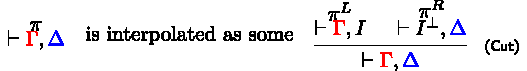
\includegraphics[width=0.95\linewidth,height=0.45\textheight,keepaspectratio]{graphic-05.pdf}\end{center}
 .\par
 
% END S4.I1.ix2.p4
   
% END S4.SS1.p2
 
% BEGIN S4.SS1.p3
 
Ultimately, one therefore builds a cut formula $I$ and two cut-free proofs $\pi_{1}$ and $\pi_{2}$ such that $I$ is an interpolant of the conclusion sequent with respect to the original splitting and such that ${\text{\scriptsize$(\mathsf{Cut})$}}(\pi_{1},\pi_{2})\longrightarrow_{\mathsf{cut}}^{\star}\pi$, a condition which is satisfied by construction.\par
 
% END S4.SS1.p3
 
% BEGIN S4.SS1.p4
 
To state precisely the properties of the two phases, we introduce the following notions:\par
  
\par\noindent  $\blacksquare$ 
% BEGIN S4.I2.i1.p1
 
A decorated proof is an $\mathsf{LL}$ proof such that each sequent is equipped with a splitting.\par
 
% END S4.I2.i1.p1
 
 
\par\noindent  $\blacksquare$ 
% BEGIN S4.I2.i2.p1
 
A coherent decorated proof is such that for each node, the splitting of the conclusion and of its premises is coherent with respect to the ancestor relation: a formula belonging to the left (resp. right) component of the splitting has all its ancestors belonging to the left (resp. right) component of the splitting. We shall now consider only such coherent proofs.\par
 
% END S4.I2.i2.p1
 
  
% END S4.SS1.p4
 
% BEGIN S4.SS1.p5
 
With the above notions, the following lemma is clear by induction on the proof:\par
 
% END S4.SS1.p5
 
% BEGIN Thmtheorem7
 
\par\medskip\noindent\textbf{Lemma 7.}\par
 
% BEGIN Thmtheorem7.p1
 
For any $\mathsf{LL}$ proof and any splitting of its conclusion sequent, the ascending phase terminates with a coherent decorated proof.\par
 
% END Thmtheorem7.p1
 
% END Thmtheorem7
 
% END S4.SS1
 
% BEGIN S4.SS2
 
\par\medskip\noindent\textbf{4.2 PRIS: Proof-Relevant Interpolation Situation}\par
 
% BEGIN S4.SS2.p1
 
We shall now focus on the top-down phase and, in order to make formal the discussion above, we shall introduce a useful class of coherent decorated proofs, called $\mathsf{PRIS}$ for proof-relevant interpolation situation; they are essentially partially solved interpolation problems:\par
 
% END S4.SS2.p1
 
% BEGIN Thmtheorem8
 
\par\medskip\noindent\textbf{Definition 8 (Proof-relevant Interpolation Situation).}\par
 
% BEGIN Thmtheorem8.p1
 
A $\mathsf{PRIS}$ for $(\Gamma,\Delta)$ is the data of:\par
  
\par\noindent  $\blacksquare$ 
% BEGIN S4.I3.i1.p1
 
the goal, that is a cut-free $\mathsf{LL}$ proof $\pi$ of conclusion $\vdash{\color[rgb]{1,0,0}\definecolor[named]{pgfstrokecolor}{rgb}{1,0,0}{{\Gamma}}},{\color[rgb]{0,0,1}\definecolor[named]{pgfstrokecolor}{rgb}{0,0,1}{{\Delta}}}$ and with $n\geq 0$ open premises $(\vdash{\color[rgb]{1,0,0}\definecolor[named]{pgfstrokecolor}{rgb}{1,0,0}{{\Gamma_{i}}}},{\color[rgb]{0,0,1}\definecolor[named]{pgfstrokecolor}{rgb}{0,0,1}{{\Delta_{i}}}})_{1\leq i\leq n}$ such that for each $1\leq i\leq n$ the formulas in $\Gamma_{i}$ (resp. $\Delta_{i}$) are ancestors of formulas in $\Gamma$ (resp. of $\Delta$);\par
 
% END S4.I3.i1.p1
 
 
\par\noindent  $\blacksquare$ 
% BEGIN S4.I3.i2.p1
 
the partial interpolants, that is for each $1\leq i\leq n$, a formula $I_{i}$ st. $\mathbb{V}\mathsf{oc}^{+}{(I_{i})}\subseteq\mathbb{V}\mathsf{oc}^{-}{(\Gamma_{i})}\cap\mathbb{V}\mathsf{oc}^{+}{(\Delta_{i})}$ and $\mathbb{V}\mathsf{oc}^{-}{(I_{i})}\subseteq\mathbb{V}\mathsf{oc}^{+}{(\Gamma_{i})}\cap\mathbb{V}\mathsf{oc}^{-}{(\Delta_{i})}$ and;\par
 
% END S4.I3.i2.p1
 
 
\par\noindent  $\blacksquare$ 
% BEGIN S4.I3.i3.p1
 
the partial solutions, that is, for each $1\leq i\leq n$, derivations $\pi_{i}^{L}$ (resp. $\pi_{i}^{R}$) of conclusion $\vdash\Gamma_{i},I_{i}$ (resp. $\vdash I_{i}^{\perp},\Delta_{i}$).\par
 
% END S4.I3.i3.p1
 
  
% END Thmtheorem8.p1
 
% END Thmtheorem8
 
% BEGIN S4.SS2.p2
 
A $\mathsf{PRIS}$ as given by the above definition will be graphically represented as in Figure 2.\par
 
% END S4.SS2.p2
 
% BEGIN S4.F2

\begin{center}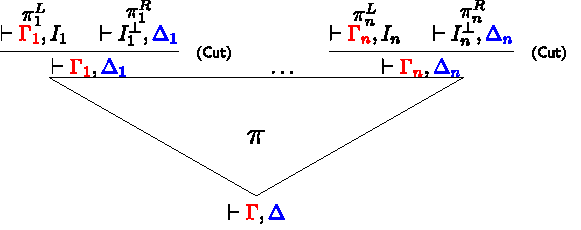
\includegraphics[width=0.95\linewidth,height=0.45\textheight,keepaspectratio]{graphic-06.pdf}\end{center}
 
Figure 2: A $\mathsf{PRIS}$– Proof-relevant Interpolation Situation.\par
 
% END S4.F2
 
% BEGIN S4.SS2.p3
 
In order to make clear our methodology of exploiting $\mathsf{PRIS}$, we define some special cases of $\mathsf{PRIS}$ which have a specific role in the forthcoming development:\par
 
% END S4.SS2.p3
 
% BEGIN Thmtheorem9
 
\par\medskip\noindent\textbf{Definition 9 (Initial, solved, and elementary $\mathsf{PRIS}$).}\par
 
% BEGIN Thmtheorem9.p1
 
We define the following cases of $\mathsf{PRIS}$:\par
  
\par\noindent  $\blacksquare$ 
% BEGIN S4.I4.i1.p1
 
An initial $\mathsf{PRIS}$ is a $\mathsf{PRIS}$ with $n=0$. It thus has the following form:\par
    
\begin{center}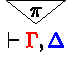
\includegraphics[width=0.95\linewidth,height=0.45\textheight,keepaspectratio]{graphic-07.pdf}\end{center}
    
with $\pi$ being a cut-free coherent decorated proof. This is the initial situation of an interpolation problem.\par
 
% END S4.I4.i1.p1
 
 
\par\noindent  $\blacksquare$ 
% BEGIN S4.I4.i2.p1
 
A solved $\mathsf{PRIS}$ is a $\mathsf{PRIS}$ with $n=1$ and $\pi$ being reduced to the trivial derivation constituted only of an open premise node $\vdash{\color[rgb]{1,0,0}\definecolor[named]{pgfstrokecolor}{rgb}{1,0,0}{{\Gamma}}},{\color[rgb]{0,0,1}\definecolor[named]{pgfstrokecolor}{rgb}{0,0,1}{{\Delta}}}$, of the form:\par
 
% END S4.I4.i2.p1
 
% BEGIN S4.I4.i2.p2
 
\begin{center}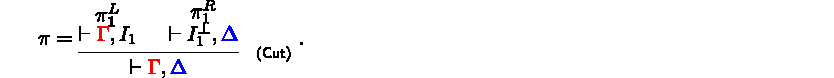
\includegraphics[width=0.95\linewidth,height=0.45\textheight,keepaspectratio]{graphic-08.pdf}\end{center}
 
% END S4.I4.i2.p2
 
% BEGIN S4.I4.i2.p3
 
A solved $\mathsf{PRIS}$ therefore corresponds to the solution of an interpolation problem, with $I_{1}$ being the interpolant and $\pi^{L}_{1},\pi^{R}_{1}$ being the interpolating proofs.\par
 
% END S4.I4.i2.p3
 
 
\par\noindent  $\blacksquare$ 
% BEGIN S4.I4.i3.p1
 
An elementary $\mathsf{PRIS}$ is a $\mathsf{PRIS}$ such that its goal is reduced to an instance of a single $n$-ary inference rule $(\mathsf{r})$, together with $n$ open premises: it is a $\mathsf{PRIS}$ where there remains a single inference rule to solve in order to obtain a solution to an interpolation problem. It thus has the form:\par
 
% END S4.I4.i3.p1
 
% BEGIN S4.I4.i3.p2
 
\begin{center}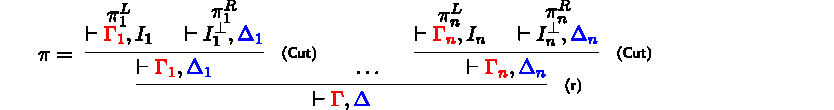
\includegraphics[width=0.95\linewidth,height=0.45\textheight,keepaspectratio]{graphic-09.pdf}\end{center}
 
% END S4.I4.i3.p2
 
  
% END Thmtheorem9.p1
 
% END Thmtheorem9
 
% END S4.SS2
 
% BEGIN S4.SS3
 
\par\medskip\noindent\textbf{4.3 Solving PRIS}\par
 
% BEGIN S4.SS3.p1
 
Our proof-relevant interpolation problem can therefore be rephrased as: How to relate initial and solved $\mathsf{PRIS}$ via cut-introduction? The crucial step lies in the following lemma:\par
 
% END S4.SS3.p1
 
% BEGIN Thmtheorem10
 
\par\medskip\noindent\textbf{Lemma 10.}\par
 
% BEGIN Thmtheorem10.p1
 
For any $n$-ary inference rule $(\mathsf{r})$ and any elementary $\mathsf{PRIS}$ $\pi$ of the form:\par
 
% END Thmtheorem10.p1
 
% BEGIN Thmtheorem10.p2
 
\begin{center}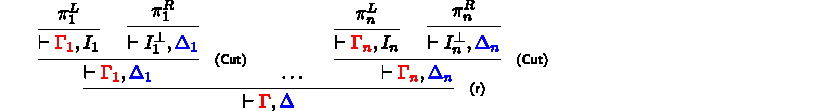
\includegraphics[width=0.95\linewidth,height=0.45\textheight,keepaspectratio]{graphic-10.pdf}\end{center}
 
% END Thmtheorem10.p2
 
% BEGIN Thmtheorem10.p3
 
there exist $I,\pi^{L},\pi^{R}$ such that 
\begin{center}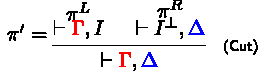
\includegraphics[width=0.95\linewidth,height=0.45\textheight,keepaspectratio]{graphic-11.pdf}\end{center}
 is a solved $\mathsf{PRIS}$ and $\pi\longleftarrow^{\star}_{\mathsf{cut}}\pi^{\prime}$.\par
 
% END Thmtheorem10.p3
 
% END Thmtheorem10
 
% BEGIN S4.SS3.p2
 
Since, each application of the above lemma reduces by one inference the size of the goal part of an interpolation situation, each sequence of cut-introduction obtained by application of Lemma 10 terminates in a solved $\mathsf{PRIS}$, that is an interpolated proof. As a conclusion, we obtain the following corollary:\par
 
% END S4.SS3.p2
 
% BEGIN Thmtheorem11
 
\par\medskip\noindent\textbf{Corollary 11.}\par
 
% BEGIN Thmtheorem11.p1
 
Any initial $\mathsf{PRIS}$ can be reduced, by cut-expansions, to a solved $\mathsf{PRIS}$.\par
 
% END Thmtheorem11.p1
 
% END Thmtheorem11
 
% BEGIN S4.SS3.p3
 
As a conclusion, we obtain the expected main theorem (Theorem 5) by working in a reversed way, using cut-introduction:\par
 
% END S4.SS3.p3
 
% BEGIN Thmtheorem12
 
\par\medskip\noindent\textbf{Theorem 12.}\par
 
% BEGIN Thmtheorem12.p1
 
Let $A,B$ be $\mathsf{LL}$ formulas and $\pi$ be a cut-free $\mathsf{LL}$ proof of $A\vdash B$.\par
 
% END Thmtheorem12.p1
 
% BEGIN Thmtheorem12.p2
 
There exists a $\mathsf{LL}$ formula $C$ such that $\mathbb{V}\mathsf{oc}^{+}{(C)}\subseteq\mathbb{V}\mathsf{oc}^{+}{(A)}\cap\mathbb{V}\mathsf{oc}^{+}{(B)}$ and $\mathbb{V}\mathsf{oc}^{-}{(C)}\subseteq\mathbb{V}\mathsf{oc}^{-}{(A)}\cap\mathbb{V}\mathsf{oc}^{-}{(B)}$ and two cut-free $\mathsf{LL}$ proofs $\pi_{1},\pi_{2}$ of $A\vdash C$ and $C\vdash B$ respectively such that 
\begin{center}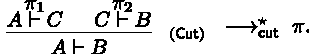
\includegraphics[width=0.95\linewidth,height=0.45\textheight,keepaspectratio]{graphic-12.pdf}\end{center}\par
 
% END Thmtheorem12.p2
 
% END Thmtheorem12
 
% END S4.SS3
 
% BEGIN S4.SS4
 
\par\medskip\noindent\textbf{4.4  Proof of Lemma 10}\par
 
% BEGIN S4.SS4.p1
 
We now prove the main lemma (missing cases are treated in Appendix A) which proceed by a case analysis on the elementary $\mathsf{PRIS}$ under consideration.\par
 
% END S4.SS4.p1
 
% BEGIN S4.SS4.SSS1
 
\par\medskip\noindent\textbf{4.4.1 Axiom case}\par
 
% BEGIN S4.SS4.SSS1.p1
  
\par\noindent  $\blacksquare$ 
% BEGIN S4.I5.i1.p1
 
If 
\begin{center}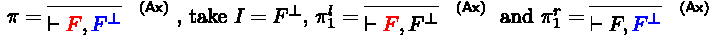
\includegraphics[width=0.95\linewidth,height=0.45\textheight,keepaspectratio]{graphic-13.pdf}\end{center}
 .\par
 
% END S4.I5.i1.p1
 
% BEGIN S4.I5.i1.p2
 
The cut between $\pi^{l}_{1}$ and $\pi^{r}_{1}$ reduces to $\pi$ by one cut-axiom reduction step.\par
 
% END S4.I5.i1.p2
 
 
\par\noindent  $\blacksquare$ 
% BEGIN S4.I5.i2.p1
 
If 
\begin{center}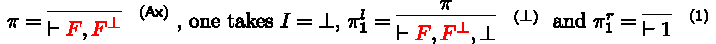
\includegraphics[width=0.95\linewidth,height=0.45\textheight,keepaspectratio]{graphic-43.pdf}\end{center}
 .\par
 
% END S4.I5.i2.p1
 
% BEGIN S4.I5.i2.p2
 
The cut of $\pi^{l}_{1}$ and $\pi^{r}_{1}$ reduces to $\pi$ by a key $1/\bot$ case.\par
 
% END S4.I5.i2.p2
 
 
\par\noindent  $\blacksquare$ 
% BEGIN S4.I5.i3.p1
 
The two other cases are treated similarly.\par
 
% END S4.I5.i3.p1
 
  
% END S4.SS4.SSS1.p1
 
% END S4.SS4.SSS1
 
% BEGIN S4.SS4.SSS2
 
\par\medskip\noindent\textbf{4.4.2 Logical rules}\par
 
% BEGIN S4.SS4.SSS2.p1
 
We analyze the possible cases for a logical rule involved in an elementary $\mathsf{PRIS}$. Note that in each case, the principal formula may be part of the left or right part of the splitting; we treat only one case each time since the other is symmetrical be taking the dual interpolant and exchanging $\pi^{L}$ and $\pi^{R}$.\par
  If the last rule is $(\mathsf{\bindnasrepma})$,  
% BEGIN S4.I6.ix1.p1
 
ie. if 
\begin{center}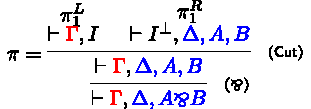
\includegraphics[width=0.95\linewidth,height=0.45\textheight,keepaspectratio]{graphic-15.pdf}\end{center}
 then taking $I^{\prime}=I$, $\pi^{L}=\pi_{1}^{L}$ and 
\begin{center}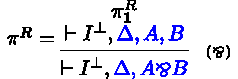
\includegraphics[width=0.95\linewidth,height=0.45\textheight,keepaspectratio]{graphic-16.pdf}\end{center}
 we obtain a solved $\mathsf{PRIS}$ $\pi^{\prime}$ such that $\pi\longleftarrow_{\mathsf{cut}}\pi^{\prime}$ by a commutative reduction of $(\mathsf{Cut})$.\par
 
% END S4.I6.ix1.p1
  If the last rule is $(\mathsf{\otimes})$,  
% BEGIN S4.I6.ix2.p1
 
ie. if 
\begin{center}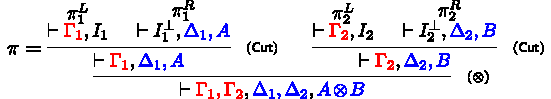
\includegraphics[width=0.95\linewidth,height=0.45\textheight,keepaspectratio]{graphic-17.pdf}\end{center}
 , then setting $I=I_{1}\hskip-1.0pt\otimes\hskip-1.0ptI_{2}$, 
\begin{center}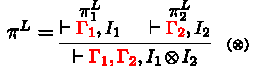
\includegraphics[width=0.95\linewidth,height=0.45\textheight,keepaspectratio]{graphic-18.pdf}\end{center}
 , 
\begin{center}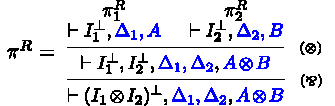
\includegraphics[width=0.95\linewidth,height=0.45\textheight,keepaspectratio]{graphic-19.pdf}\end{center}
 one gets a solved $\mathsf{PRIS}$ $\pi^{\prime}$ such that $\pi\longleftarrow^{\star}_{\mathsf{cut}}\pi^{\prime}$ by a commutative reduction of $(\mathsf{Cut})$ and a key ${\text{\scriptsize$(\mathsf{\otimes})$}}/{\text{\scriptsize$(\mathsf{\bindnasrepma})$}}$ case.\par
 
% END S4.I6.ix2.p1
  If the last rule is $(\mathsf{!p})$,  
% BEGIN S4.I6.ix3.p1
 
that is 
\begin{center}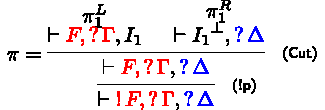
\includegraphics[width=0.95\linewidth,height=0.45\textheight,keepaspectratio]{graphic-20.pdf}\end{center}
 , then by setting 
\begin{center}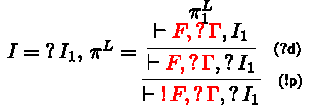
\includegraphics[width=0.95\linewidth,height=0.45\textheight,keepaspectratio]{graphic-21.pdf}\end{center}
 and 
\begin{center}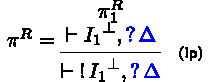
\includegraphics[width=0.95\linewidth,height=0.45\textheight,keepaspectratio]{graphic-22.pdf}\end{center}
 , one gets that $\pi$ cut-expands to $\pi^{\prime}$: 
\begin{center}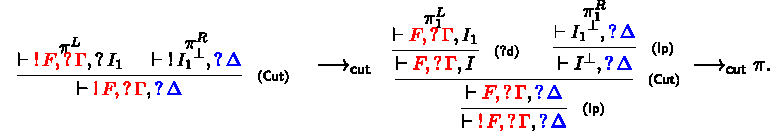
\includegraphics[width=0.95\linewidth,height=0.45\textheight,keepaspectratio]{graphic-23.pdf}\end{center}\par
 
% END S4.I6.ix3.p1
  If the last rule is $(\mathsf{?c})$,  
% BEGIN S4.I6.ix4.p1
 
ie. 
\begin{center}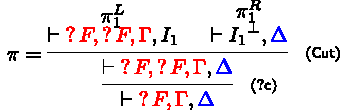
\includegraphics[width=0.95\linewidth,height=0.45\textheight,keepaspectratio]{graphic-70.pdf}\end{center}
 , by setting $I=I_{1}$, $\pi^{R}=\pi^{R}_{1}$ and 
\begin{center}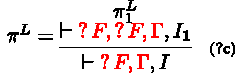
\includegraphics[width=0.95\linewidth,height=0.45\textheight,keepaspectratio]{graphic-71.pdf}\end{center}
 one gets that $\pi$ cut-expands to the solved $\mathsf{PRIS}$ $\pi^{\prime}$:\par
 
% END S4.I6.ix4.p1
 
% BEGIN S4.I6.ix4.p2
 
\begin{center}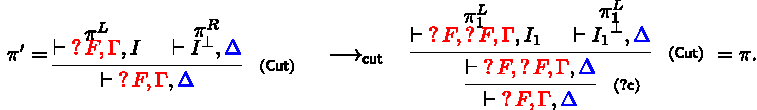
\includegraphics[width=0.95\linewidth,height=0.45\textheight,keepaspectratio]{graphic-26.pdf}\end{center}
 
% END S4.I6.ix4.p2
  If the last rule is $(\mathsf{\exists})$,  
% BEGIN S4.I6.ix5.p1
 
ie. 
\begin{center}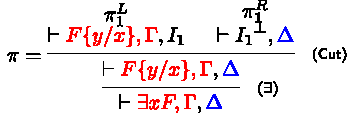
\includegraphics[width=0.95\linewidth,height=0.45\textheight,keepaspectratio]{graphic-27.pdf}\end{center}
 with the vocabulary condition $\mathbb{V}\mathsf{oc}{(I_{1})}\subseteq\mathbb{V}\mathsf{oc}{(F\{y/x\},\Gamma)}\cap\mathbb{V}\mathsf{oc}(\Delta)$. In this case, note that we treat only the case of a FO language containing no function symbols. We reason by case on whether $y$ occurs in $\Gamma,\Delta$:\par
  
\par\noindent  $\blacksquare$ 
% BEGIN S4.I6.ix5.I1.i1.p1
 
If $y$ occurs in both, then we simply take $I=I_{1}$ as interpolant, 
\begin{center}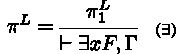
\includegraphics[width=0.95\linewidth,height=0.45\textheight,keepaspectratio]{graphic-28.pdf}\end{center}
 and $\pi^{R}=\pi^{R}_{1}$. Since $\mathbb{V}\mathsf{oc}(I)=\mathbb{V}\mathsf{oc}{(I_{1})}\subseteq\mathbb{V}\mathsf{oc}{(F,\Gamma)}\cap\mathbb{V}\mathsf{oc}(\Delta)=\mathbb{V}\mathsf{oc}{(\exists xF,\Gamma)}\cap\mathbb{V}\mathsf{oc}(\Delta)$, we have that 
\begin{center}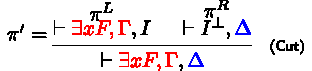
\includegraphics[width=0.95\linewidth,height=0.45\textheight,keepaspectratio]{graphic-32.pdf}\end{center}
 is a solved $\mathsf{PRIS}$ to which $\pi$ cut-expands via a cut-commutation rule.\par
 
% END S4.I6.ix5.I1.i1.p1
 
 
\par\noindent  $\blacksquare$ 
% BEGIN S4.I6.ix5.I1.i2.p1
 
If $y$ occurs in $\Gamma$ but not in $\Delta$, then we set $I=\exists yI_{1}$, 
\begin{center}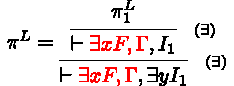
\includegraphics[width=0.95\linewidth,height=0.45\textheight,keepaspectratio]{graphic-30.pdf}\end{center}
 and 
\begin{center}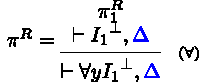
\includegraphics[width=0.95\linewidth,height=0.45\textheight,keepaspectratio]{graphic-31.pdf}\end{center}
 we have that 
\begin{center}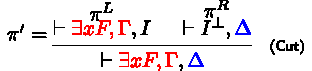
\includegraphics[width=0.95\linewidth,height=0.45\textheight,keepaspectratio]{graphic-32.pdf}\end{center}
 is a solved $\mathsf{PRIS}$ to which $\pi$ cut-expands via a cut-commutation rule and a key ${\text{\scriptsize$(\mathsf{\exists})$}}/{\text{\scriptsize$(\mathsf{\forall})$}}$ rule:\par
 
% END S4.I6.ix5.I1.i2.p1
 
% BEGIN S4.I6.ix5.I1.i2.p2
 
\begin{center}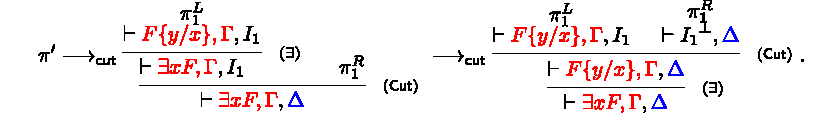
\includegraphics[width=0.95\linewidth,height=0.45\textheight,keepaspectratio]{graphic-33.pdf}\end{center}
 
% END S4.I6.ix5.I1.i2.p2
 
 
\par\noindent  $\blacksquare$ 
% BEGIN S4.I6.ix5.I1.i3.p1
 
If $y$ occurs in $\Delta$ but not in $\Gamma$, then we set $I=\forall yI_{1}$, 
\begin{center}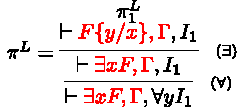
\includegraphics[width=0.95\linewidth,height=0.45\textheight,keepaspectratio]{graphic-34.pdf}\end{center}
 and 
\begin{center}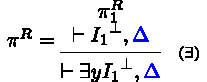
\includegraphics[width=0.95\linewidth,height=0.45\textheight,keepaspectratio]{graphic-35.pdf}\end{center}
 . One gets that 
\begin{center}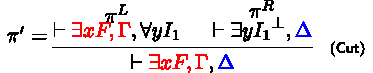
\includegraphics[width=0.95\linewidth,height=0.45\textheight,keepaspectratio]{graphic-36.pdf}\end{center}
 is a solved $\mathsf{PRIS}$ to which $\pi$ cut-expands: 
\begin{center}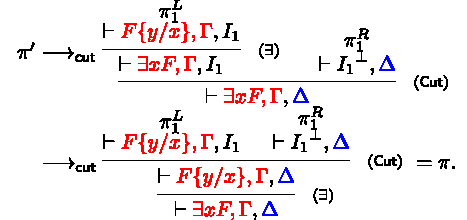
\includegraphics[width=0.95\linewidth,height=0.45\textheight,keepaspectratio]{graphic-37.pdf}\end{center}\par
 
% END S4.I6.ix5.I1.i3.p1
 
  
% END S4.I6.ix5.p1
  Other cases  
% BEGIN S4.I6.ix6.p1
 
are treated similarly.\par
 
% END S4.I6.ix6.p1
   
% END S4.SS4.SSS2.p1
 
% END S4.SS4.SSS2
 
% END S4.SS4
 
% BEGIN S4.SS5
 
\par\medskip\noindent\textbf{4.5 Some consequences and extensions}\par
 
% BEGIN S4.SS5.p1
 
In the same way as in the previous section, a similar development of $\mathsf{LK}$-PRIS and $\mathsf{LJ}$-PRIS can be done, either from scratch or by means of linear embeddings which relates linear $\mathsf{PRIS}$ to classicial or intuitionistic ones, this results in the following proposition:\par
 
% END S4.SS5.p1
 
% BEGIN Thmtheorem13
 
\par\medskip\noindent\textbf{Proposition 13.}\par
 
% BEGIN Thmtheorem13.p1
 
Any initial $\mathsf{LK}$-PRIS (resp. $\mathsf{LJ}$-PRIS) can be reduced, by cut-expansions, to a solved $\mathsf{LK}$-PRIS (resp. solved $\mathsf{LJ}$-PRIS).\par
 
% END Thmtheorem13.p1
 
% END Thmtheorem13
 
% BEGIN Thmtheorem14
 
\par\medskip\noindent\textbf{$\blacktriangleright$ Remark 14.}\par
 
% BEGIN Thmtheorem14.p1
 
In fact, the above theorem does not rely on the cut-freeness of $\pi$, only the notion of interpolant does: the cut-introduction performed in solving $\mathsf{PRIS}$ can indeed be extended to handle the cut-case, as long as one relaxes the conditions on the language for the interpolant. This suggests an immediate generalization of proof-relevant Craig and Lyndon’s interpolation for proofs with cuts in which each (pair of) cut-formula is assigned to the left/right component of a splitting (in a consistent way for a given cut inference): the language of the interpolant is then constructed by taking into account the language of the cut-formulas depending on the choice of splitting. In that case, an additional degree of freedom appears in the choice of the interpolant when assigning each cut to a component of the splitting: strategies for optimizing the language of the interpolant could therefore be investigated.\par
 
% END Thmtheorem14.p1
 
% END Thmtheorem14
 
% BEGIN Thmtheorem15
 
\par\medskip\noindent\textbf{$\blacktriangleright$ Remark 15.}\par
 
% BEGIN Thmtheorem15.p1
 
Complementing on the previous remark, analytic cuts (that is cut formulas that are subformula of some formula of the conclusion sequent) are of particular interest here. Indeed, the above described procedure to work with $\mathsf{PRIS}$ containing cuts can be readily applied to proofs with analytic cuts.\par
 
% END Thmtheorem15.p1
 
% BEGIN Thmtheorem15.p2
 
In a similar way, it would be interesting to consider extending our procedure to proofs with cuts which are globally analytic (ie. simply requiring that every cut-formula is a subformula of some formula in the conclusion sequent). While the vocabulary constraint on interpolant is locally violated when encountering a globally-analytic cut, it is globally satisfied when reaching a solved $\mathsf{PRIS}$. Other weakenings on the conditions on cut-formulas car be considered, such as the semi-analyticity conditions by Jalali and Tabatakai [38].\par
 
% END Thmtheorem15.p2
 
% END Thmtheorem15
 
% END S4.SS5
 
% END S4



% BEGIN S5
 
\par\medskip\noindent\textbf{5 On the computational significance of the result: Interpolating System L}\par
 
% BEGIN S5.p1
 
Stated purely in terms of interpolating validity judgements, interpolation is not very meaningful computationally of course. On the other hand, the refined statement investigated in the present paper opens new perspectives: the interpolant formula can be viewed as a an interface type $I$ through which a computation can from data type $A$ to data type $B$ be factored via type $I$. Let us focus on intuitionistic statement (say, in $\mathsf{ILL}$ or $\mathsf{LJ}$):\par
 
% END S5.p1
 
% BEGIN S5.p2
 
If $\pi$ proves $\Gamma,\Delta\vdash C$, there exists some formula $I$ such that $\mathbb{V}\mathsf{oc}(I)\subseteq\mathbb{V}\mathsf{oc}{(\Gamma)}\cap\mathbb{V}\mathsf{oc}{(\Delta,C)}$ and proofs $\pi_{1},\pi_{2}$ of $\Gamma\vdash I$ and $I,\Delta\vdash C$ respectively, such that ${\text{\scriptsize$(\mathsf{Cut})$}}(\pi_{1},\pi_{2})\longrightarrow_{\mathsf{cut}}^{\star}\pi$.\par
 
% END S5.p2
 
% BEGIN S5.p3
 
Rephrased in terms of the $\lambda$-calculus, that would mean in particular that: for any closed term $\lambda x.t:A\rightarrow B$ there is a type $C$ such that $\mathbb{V}\mathsf{oc}(C)\subseteq\mathbb{V}\mathsf{oc}(A)\cap\mathbb{V}\mathsf{oc}(B)$ and terms $u:A\rightarrow C$ and $v:C\rightarrow B$ such that $\lambda x.t=_{\beta}\lambda x.(v(ux))$. This is the content of the analysis by Čubrić. Data type $C$ can therefore be viewed as an interface between types $A$ and $B$ while processing computation $t$, involving only pieces of data involved in both $A$ and $B$.\par
 
% END S5.p3
 
% BEGIN S5.p4
 
Of course, this interface depends in $t$ itself in the above proof, which would be different if uniform interpolation is lifted to this proof-relevant framework. Indeed, in that case, the data type for the interpolant only depend on $A$ and the common vocabulary with the output type. In that way, interpolation would express some generic preprocessing from $A$ to the interpolant type $UI(A,\mathcal{V})$ depending only on formula A and type variables $\mathcal{V}$, from which any computation to a type $B$ (sharing vocabulary $\mathcal{V}$ with $A$) can be performed. In the same spirit, more precise results on interpolation (especially on polarity of occurrences of relational symbols, etc.) would provide more information on data usage.\par
 
% END S5.p4
 
% BEGIN S5.p5
  
% END S5.p5
 
% BEGIN S5.p6
 
We shall now outline a rephrasing of our previous results in a term calculus which corresponds to sequent calculus as the $\lambda$-calculus does to natural deduction. For uniformity, this version is essentially inspired from the calculus designed by Munch-Maccagnoni [29, 30], presented in a two-sided manner rather than one-sided to emphasize the input/output behaviour and term/context duality, that we restrict to the purely linear (ie multiplicative and additive setting).\par
 
% END S5.p6
 
% BEGIN Thmtheorem16
 
\par\medskip\noindent\textbf{Definition 16 (Linear System L).}\par
 
% BEGIN Thmtheorem16.p1
 
As usual, the grammar and type system of linear system L consists of three syntactic categories: commands, terms and contexts, defined by mutual recursion:\par
  
\par\noindent  $\blacksquare$ 
% BEGIN S5.I1.i1.p1
 
$c::=\langle t\mid e\rangle$\par
 
% END S5.I1.i1.p1
 
 
\par\noindent  $\blacksquare$ 
% BEGIN S5.I1.i2.p1
 
$t,u::=x\mid\mu\alpha.c\mid(s,t)\mid\lambda x.t\mid\mu[\alpha,\beta].c\mid()\mid\mu[].c\mid\iota_{1}(t)\mid\iota_{2}(t)\mid\mu(\pi_{1}(\alpha)\mapsto c\mid\pi_{2}(\beta)\mapsto d)\mid{{\tt tp}}$\par
 
% END S5.I1.i2.p1
 
 
\par\noindent  $\blacksquare$ 
% BEGIN S5.I1.i3.p1
 
$e,f::=\alpha\mid\tilde{\mu}x.c\mid\tilde{\mu}(x,y).c\mid t\cdot e\mid[e,f]\mid\tilde{\mu}().c\mid[]\mid\pi_{1}(e)\mid\pi_{2}(e)\mid\tilde{\mu}(\iota_{1}(x)\mapsto c\mid\iota_{2}(x)\mapsto d)\mid{{\tt stop}}$\par
 
% END S5.I1.i3.p1
 
  
This gives rise to three kinds of typing judgments: $c:(\Gamma\vdash\Delta);\quad\Gamma\vdash t:A\mid\Delta;\quad\Gamma\mid e:A\vdash\Delta$ and the typing rules given in Figure 3.\par
 
% END Thmtheorem16.p1
 
% END Thmtheorem16
 
% BEGIN S5.F3

\begin{center}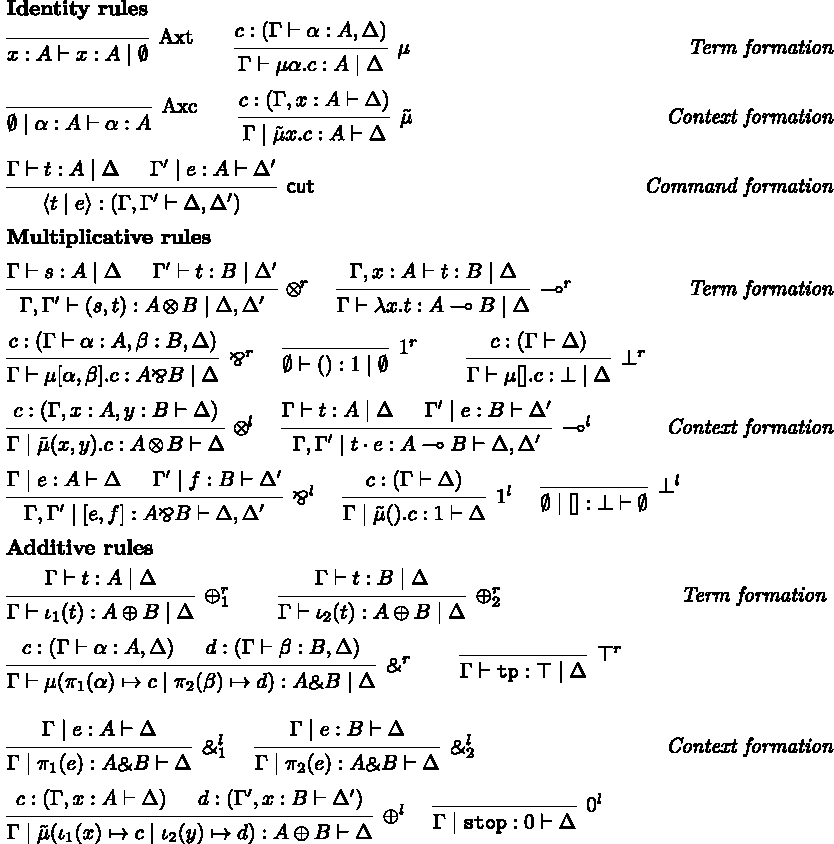
\includegraphics[width=0.95\linewidth,height=0.45\textheight,keepaspectratio]{graphic-38.pdf}\end{center}
 
Figure 3: Type derivation rules for System $\mathsf{L}$.\par
 
% END S5.F3
 
% BEGIN Thmtheorem17
 
\par\medskip\noindent\textbf{$\blacktriangleright$ Remark 17.}\par
 
% BEGIN Thmtheorem17.p1
 
Notice that we use very similar notation for term and context constructs ($\iota/\pi$, $(u,v)/[e,f]$, $()/[]$, ${\tt tp}/{\tt stop}$), in order to emphasize the deep symmetry of the System ${\mathsf{L}}$ framework we work with. This symmetry is exploited in the proof of our main theorem.\par
 
% END Thmtheorem17.p1
 
% BEGIN Thmtheorem17.p2
 
The calculus could actually be presented with one-sided typing judgments, see [29].\par
 
% END Thmtheorem17.p2
 
% END Thmtheorem17
 
% BEGIN S5.p7
 
We provide some of the main reduction rules of this calculus, keeping in mind the invariant that one reduces commands:\par
  
\par\noindent  $\blacksquare$ 
% BEGIN S5.I2.i1.p1
 
$\langle\mu\alpha.c\mid e\rangle\longrightarrow_{\mu}c\{e/\alpha\}$\par
 
% END S5.I2.i1.p1
 
 
\par\noindent  $\blacksquare$ 
% BEGIN S5.I2.i2.p1
 
$\langle t\mid\tilde{\mu}x.c\rangle\longrightarrow_{\tilde{\mu}}c\{t/x\}$\par
 
% END S5.I2.i2.p1
 
 
\par\noindent  $\blacksquare$ 
% BEGIN S5.I2.i3.p1
 
$\langle\lambda x.t\mid u\cdot e\rangle\longrightarrow_{\lambda}\langle\tilde{\mu}x.\langle t\mid e\rangle\mid u\rangle$\par
 
% END S5.I2.i3.p1
 
 
\par\noindent  $\blacksquare$ 
% BEGIN S5.I2.i4.p1
 
$\langle(t,u)\mid\tilde{\mu}(x,y).c\rangle\longrightarrow_{\hskip-1.0pt\otimes\hskip-1.0pt}c\{t/x,u/y\}$\par
 
% END S5.I2.i4.p1
 
 
\par\noindent  $\blacksquare$ 
% BEGIN S5.I2.i5.p1
 
$\langle\mu[\alpha,\beta].c\mid[e,f]\rangle\longrightarrow_{\bindnasrepma}c\{e/\alpha,f/\beta\}$\par
 
% END S5.I2.i5.p1
 
 
\par\noindent  $\blacksquare$ 
% BEGIN S5.I2.i6.p1
 
$\langle\iota_{j}(t)\mid\tilde{\mu}(\iota_{1}(x_{1})\mapsto c_{1}\mid\iota_{2}(x_{2})\mapsto c_{2})\rangle\longrightarrow_{\oplus}c_{j}\{t/x_{j}\}$\par
 
% END S5.I2.i6.p1
 
 
\par\noindent  $\blacksquare$ 
% BEGIN S5.I2.i7.p1
 
$\langle\mu(\pi_{1}(\alpha_{1})\mapsto c_{1}\mid\pi_{2}(\alpha_{2})\mapsto c_{2})\mid\pi_{j}(e)\rangle\longrightarrow_{\binampersand}c_{j}\{e/\alpha_{j}\}$\par
 
% END S5.I2.i7.p1
 
 
\par\noindent  $\blacksquare$ 
% BEGIN S5.I2.i8.p1
 
$\langle()\mid\tilde{\mu}().c\rangle\longrightarrow_{1}c$\par
 
% END S5.I2.i8.p1
 
 
\par\noindent  $\blacksquare$ 
% BEGIN S5.I2.i9.p1
 
$\langle\mu[].c\mid[]\rangle\longrightarrow_{\bot}c$\par
 
% END S5.I2.i9.p1
 
  
% END S5.p7
 
% BEGIN S5.p8
 
Moreover, one shall consider in the development below the $\eta$ rules for $\mu$ and $\tilde{\mu}$ (which respectively reduce terms and contexts):\par
  
\par\noindent  $\blacksquare$ 
% BEGIN S5.I3.i1.p1
 
${\mu\alpha.\langle t\mid\alpha\rangle}\longrightarrow_{\eta_{\mu}}t$ (if $\alpha$ is not free in $t$)\par
 
% END S5.I3.i1.p1
 
 
\par\noindent  $\blacksquare$ 
% BEGIN S5.I3.i2.p1
 
${\tilde{\mu}x.\langle x\mid e\rangle}\longrightarrow_{\eta_{\tilde{\mu}}}e$ (if $x$ is not free in $e$)\par
 
% END S5.I3.i2.p1
 
  
% END S5.p8
 
% BEGIN S5.p9
 
The above rules satisfy the expected subject reduction property. Moreover, we need to reflect the splitting of sequents which will lead us to define a system L with a split typing system to be detailed now.\par
 
% END S5.p9
 
% BEGIN Thmtheorem18
 
\par\medskip\noindent\textbf{Definition 18 (System L with split typing judgements).}\par
 
% BEGIN Thmtheorem18.p1
 
We introduce split typing judgements where types are enriched with a splitting information in the form of a label $l\in\{L,R\}$ carried by each type occurring in the judgment, which are then of one of the following shape:\par
  
\par\noindent  $\blacksquare$ 
% BEGIN S5.I4.i1.p1
 
$c:(x_{1}:A_{1}^{k_{1}},\dots,x_{m}:A_{m}^{k_{m}}\vdash\alpha_{1}:B_{1}^{l_{1}},\dots,\alpha_{n}:B_{n}^{l_{n}})$\par
 
% END S5.I4.i1.p1
 
 
\par\noindent  $\blacksquare$ 
% BEGIN S5.I4.i2.p1
 
$x_{1}:A_{1}^{k_{1}},\dots,x_{m}:A_{m}^{k_{m}}\vdash t:B^{l}\mid\alpha_{1}:B_{1}^{l_{1}},\dots,\alpha_{n}:B_{n}^{l_{n}}$\par
 
% END S5.I4.i2.p1
 
 
\par\noindent  $\blacksquare$ 
% BEGIN S5.I4.i3.p1
 
$x_{1}:A_{1}^{k_{1}},\dots,x_{m}:A_{m}^{k_{m}}\mid e:A^{k}\vdash\alpha_{1}:B_{1}^{l_{1}},\dots,\alpha_{n}:B_{n}^{l_{n}}$\par
 
% END S5.I4.i3.p1
 
  
with $k,l,k_{1},\dots,k_{m},l_{1},\dots,l_{n}\in\{L,R\}$.\par
 
% END Thmtheorem18.p1
 
% BEGIN Thmtheorem18.p2
 
By convention, to save space and ease the reading of judgements, we may use colors to represent the labels: a labelled type $T^{L}$ (resp. $U^{R}$) may be written ${\color[rgb]{1,0,0}\definecolor[named]{pgfstrokecolor}{rgb}{1,0,0}{{T}}}$ (resp. ${\color[rgb]{0,0,1}\definecolor[named]{pgfstrokecolor}{rgb}{0,0,1}{{U}}}$), shorthand which will be extended to whole typing contexts sharing the same label: ${\color[rgb]{1,0,0}\definecolor[named]{pgfstrokecolor}{rgb}{1,0,0}{{\Gamma}}}$ or ${\color[rgb]{0,0,1}\definecolor[named]{pgfstrokecolor}{rgb}{0,0,1}{{\Gamma}}}$.\par
 
% END Thmtheorem18.p2
 
% END Thmtheorem18
  
% BEGIN Thmtheorem19
 
\par\medskip\noindent\textbf{Theorem 19.}\par
 
% BEGIN Thmtheorem19.p1
 
In what follows, $t$ (resp. $e$, resp. $c$) is a normal L-term (resp. normal L-context, resp. normal L-command). The following interpolating results hold:\par
  
\par\noindent  1. 
% BEGIN S5.I5.i1.p1
 
If $c:({\color[rgb]{1,0,0}\definecolor[named]{pgfstrokecolor}{rgb}{1,0,0}{{\Gamma_{1}}}},{\color[rgb]{0,0,1}\definecolor[named]{pgfstrokecolor}{rgb}{0,0,1}{{\Gamma_{2}}}}\vdash{\color[rgb]{1,0,0}\definecolor[named]{pgfstrokecolor}{rgb}{1,0,0}{{\Delta_{1}}}},{\color[rgb]{0,0,1}\definecolor[named]{pgfstrokecolor}{rgb}{0,0,1}{{\Delta_{2}}}})$, there exist a type $I\in\mathbb{V}\mathsf{oc}({\Gamma_{1},\Delta_{1}})\cap\mathbb{V}\mathsf{oc}({\Gamma_{2},\Delta_{2}})$ and $t,e$ such that ${\color[rgb]{1,0,0}\definecolor[named]{pgfstrokecolor}{rgb}{1,0,0}{{\Gamma_{1}}}}\vdash t:{\color[rgb]{1,0,0}\definecolor[named]{pgfstrokecolor}{rgb}{1,0,0}{{I}}}\mid{\color[rgb]{1,0,0}\definecolor[named]{pgfstrokecolor}{rgb}{1,0,0}{{\Delta_{1}}}}$ and ${\color[rgb]{0,0,1}\definecolor[named]{pgfstrokecolor}{rgb}{0,0,1}{{\Gamma_{2}}}}\mid e:{\color[rgb]{0,0,1}\definecolor[named]{pgfstrokecolor}{rgb}{0,0,1}{{I}}}\vdash{\color[rgb]{0,0,1}\definecolor[named]{pgfstrokecolor}{rgb}{0,0,1}{{\Delta_{2}}}}$, and $\langle t\mid e\rangle\longrightarrow^{\star}c$.\par
 
% END S5.I5.i1.p1
 
 
\par\noindent  2. 
% BEGIN S5.I5.i2.p1
 
If ${\color[rgb]{1,0,0}\definecolor[named]{pgfstrokecolor}{rgb}{1,0,0}{{\Gamma_{1}}}},{\color[rgb]{0,0,1}\definecolor[named]{pgfstrokecolor}{rgb}{0,0,1}{{\Gamma_{2}}}}\vdash t:{\color[rgb]{1,0,0}\definecolor[named]{pgfstrokecolor}{rgb}{1,0,0}{{A}}}\mid{\color[rgb]{1,0,0}\definecolor[named]{pgfstrokecolor}{rgb}{1,0,0}{{\Delta_{1}}}},{\color[rgb]{0,0,1}\definecolor[named]{pgfstrokecolor}{rgb}{0,0,1}{{\Delta_{2}}}}$, there exist a type $I\in\mathbb{V}\mathsf{oc}({\Gamma_{1},\Delta_{1},A})\cap\mathbb{V}\mathsf{oc}({\Gamma_{2},\Delta_{2}})$ and $\alpha,t^{\prime},e^{\prime}$ such that ${\color[rgb]{1,0,0}\definecolor[named]{pgfstrokecolor}{rgb}{1,0,0}{{\Gamma_{1}}}}\vdash t^{\prime}:{\color[rgb]{1,0,0}\definecolor[named]{pgfstrokecolor}{rgb}{1,0,0}{{A}}}\mid\alpha:{\color[rgb]{1,0,0}\definecolor[named]{pgfstrokecolor}{rgb}{1,0,0}{{I}}},{\color[rgb]{1,0,0}\definecolor[named]{pgfstrokecolor}{rgb}{1,0,0}{{\Delta_{1}}}}$ and ${\color[rgb]{0,0,1}\definecolor[named]{pgfstrokecolor}{rgb}{0,0,1}{{\Gamma_{2}}}}\mid e^{\prime}:{\color[rgb]{0,0,1}\definecolor[named]{pgfstrokecolor}{rgb}{0,0,1}{{I}}}\vdash{\color[rgb]{0,0,1}\definecolor[named]{pgfstrokecolor}{rgb}{0,0,1}{{\Delta_{2}}}}$, and $t^{\prime}\{e^{\prime}/\alpha\}\longrightarrow^{\star}t$.\par
 
% END S5.I5.i2.p1
 
 
\par\noindent  3. 
% BEGIN S5.I5.i3.p1
 
If ${\color[rgb]{1,0,0}\definecolor[named]{pgfstrokecolor}{rgb}{1,0,0}{{\Gamma_{1}}}},{\color[rgb]{0,0,1}\definecolor[named]{pgfstrokecolor}{rgb}{0,0,1}{{\Gamma_{2}}}}\mid e:{\color[rgb]{1,0,0}\definecolor[named]{pgfstrokecolor}{rgb}{1,0,0}{{A}}}\vdash{\color[rgb]{1,0,0}\definecolor[named]{pgfstrokecolor}{rgb}{1,0,0}{{\Delta_{1}}}},{\color[rgb]{0,0,1}\definecolor[named]{pgfstrokecolor}{rgb}{0,0,1}{{\Delta_{2}}}}$, there exist a type $I\in\mathbb{V}\mathsf{oc}({\Gamma_{1},\Delta_{1},A})\cap\mathbb{V}\mathsf{oc}({\Gamma_{2},\Delta_{2}})$ and $\alpha,e^{\prime},e^{\prime\prime}$ such that ${\color[rgb]{1,0,0}\definecolor[named]{pgfstrokecolor}{rgb}{1,0,0}{{\Gamma_{1}}}}\mid e^{\prime}:{\color[rgb]{1,0,0}\definecolor[named]{pgfstrokecolor}{rgb}{1,0,0}{{A}}}\mid\alpha:{\color[rgb]{1,0,0}\definecolor[named]{pgfstrokecolor}{rgb}{1,0,0}{{I}}},{\color[rgb]{1,0,0}\definecolor[named]{pgfstrokecolor}{rgb}{1,0,0}{{\Delta_{1}}}}$ and ${\color[rgb]{0,0,1}\definecolor[named]{pgfstrokecolor}{rgb}{0,0,1}{{\Gamma_{2}}}}\mid e^{\prime\prime}:{\color[rgb]{0,0,1}\definecolor[named]{pgfstrokecolor}{rgb}{0,0,1}{{I}}}\vdash{\color[rgb]{0,0,1}\definecolor[named]{pgfstrokecolor}{rgb}{0,0,1}{{\Delta_{2}}}}$, and $e^{\prime}\{e^{\prime\prime}/\alpha\}\longrightarrow^{\star}e$.\par
 
% END S5.I5.i3.p1
 
 
\par\noindent  4. 
% BEGIN S5.I5.i4.p1
 
If ${\color[rgb]{1,0,0}\definecolor[named]{pgfstrokecolor}{rgb}{1,0,0}{{\Gamma_{1}}}},{\color[rgb]{0,0,1}\definecolor[named]{pgfstrokecolor}{rgb}{0,0,1}{{\Gamma_{2}}}}\vdash t:{\color[rgb]{0,0,1}\definecolor[named]{pgfstrokecolor}{rgb}{0,0,1}{{A}}}\mid{\color[rgb]{1,0,0}\definecolor[named]{pgfstrokecolor}{rgb}{1,0,0}{{\Delta_{1}}}},{\color[rgb]{0,0,1}\definecolor[named]{pgfstrokecolor}{rgb}{0,0,1}{{\Delta_{2}}}}$, there exist a type $I\in\mathbb{V}\mathsf{oc}({\Gamma_{1},\Delta_{1}})\cap\mathbb{V}\mathsf{oc}({\Gamma_{2},\Delta_{2},A})$ and $\alpha,t^{\prime},t^{\prime\prime}$ such that ${\color[rgb]{1,0,0}\definecolor[named]{pgfstrokecolor}{rgb}{1,0,0}{{\Gamma_{1}}}}\vdash t^{\prime\prime}:{\color[rgb]{1,0,0}\definecolor[named]{pgfstrokecolor}{rgb}{1,0,0}{{I}}}\mid{\color[rgb]{1,0,0}\definecolor[named]{pgfstrokecolor}{rgb}{1,0,0}{{\Delta_{1}}}}$ and ${\color[rgb]{0,0,1}\definecolor[named]{pgfstrokecolor}{rgb}{0,0,1}{{\Gamma_{2}}}},x:{\color[rgb]{0,0,1}\definecolor[named]{pgfstrokecolor}{rgb}{0,0,1}{{I}}}\vdash t^{\prime}:{\color[rgb]{0,0,1}\definecolor[named]{pgfstrokecolor}{rgb}{0,0,1}{{A}}}\mid{\color[rgb]{0,0,1}\definecolor[named]{pgfstrokecolor}{rgb}{0,0,1}{{\Delta_{2}}}}$, and $t^{\prime}\{t^{\prime\prime}/x\}\longrightarrow^{\star}t$.\par
 
% END S5.I5.i4.p1
 
 
\par\noindent  5. 
% BEGIN S5.I5.i5.p1
 
If ${\color[rgb]{1,0,0}\definecolor[named]{pgfstrokecolor}{rgb}{1,0,0}{{\Gamma_{1}}}},{\color[rgb]{0,0,1}\definecolor[named]{pgfstrokecolor}{rgb}{0,0,1}{{\Gamma_{2}}}}\mid e:{\color[rgb]{0,0,1}\definecolor[named]{pgfstrokecolor}{rgb}{0,0,1}{{A}}}\vdash{\color[rgb]{1,0,0}\definecolor[named]{pgfstrokecolor}{rgb}{1,0,0}{{\Delta_{1}}}},{\color[rgb]{0,0,1}\definecolor[named]{pgfstrokecolor}{rgb}{0,0,1}{{\Delta_{2}}}}$, there exist a type $I\in\mathbb{V}\mathsf{oc}({\Gamma_{1},\Delta_{1}})\cap\mathbb{V}\mathsf{oc}({\Gamma_{2},\Delta_{2},A})$ and $x,t^{\prime},e^{\prime}$ such that ${\color[rgb]{1,0,0}\definecolor[named]{pgfstrokecolor}{rgb}{1,0,0}{{\Gamma_{1}}}}\vdash t^{\prime}:{\color[rgb]{1,0,0}\definecolor[named]{pgfstrokecolor}{rgb}{1,0,0}{{I}}}\mid{\color[rgb]{1,0,0}\definecolor[named]{pgfstrokecolor}{rgb}{1,0,0}{{\Delta_{1}}}}$ and ${\color[rgb]{0,0,1}\definecolor[named]{pgfstrokecolor}{rgb}{0,0,1}{{\Gamma_{2}}}},x:{\color[rgb]{0,0,1}\definecolor[named]{pgfstrokecolor}{rgb}{0,0,1}{{I}}}\mid e^{\prime}:{\color[rgb]{0,0,1}\definecolor[named]{pgfstrokecolor}{rgb}{0,0,1}{{A}}}\vdash{\color[rgb]{0,0,1}\definecolor[named]{pgfstrokecolor}{rgb}{0,0,1}{{\Delta_{2}}}}$, and $e^{\prime}\{t^{\prime}/x\}\longrightarrow^{\star}e$.\par
 
% END S5.I5.i5.p1
 
  
% END Thmtheorem19.p1
 
% END Thmtheorem19
 
% BEGIN S5.SS0.SSS0.P0.SPx1
 
\par\medskip\noindent\textbf{Proof.}\par
 
% BEGIN S5.SS0.SSS0.P0.SPx1.p1
 
The result is proved by mutual induction on the structure of terms, contexts and commands. We detail cases 1–3, case 4 (resp. 5) being essentially similar to cases 3 (resp. 2).\par
 
% END S5.SS0.SSS0.P0.SPx1.p1
 
% END S5.SS0.SSS0.P0.SPx1
 
% BEGIN S5.SS0.SSS0.P0.SPx2
 
\par\medskip\noindent\textbf{Case 1.}\par
 
% BEGIN S5.SS0.SSS0.P0.SPx2.p1
 
If $c$ is a command in normal form, it is either of the form $\langle z\mid e\rangle$ (with $z$ being declared in $\Gamma_{1}$ or $\Gamma_{2}$) or $\langle t\mid\beta\rangle$ (with $\alpha$ being declared in $\Delta_{1}$ or $\Delta_{2}$). Depending on the case and whether the variable is declared in the left or right component of the typing contexts, we apply induction hypotheses for one of cases 2–4.\par
 
% END S5.SS0.SSS0.P0.SPx2.p1
 
% BEGIN S5.SS0.SSS0.P0.SPx2.p2
 
Let us assume for instance that $c=\langle z\mid e\rangle$ and $\langle z\mid e\rangle:({\color[rgb]{1,0,0}\definecolor[named]{pgfstrokecolor}{rgb}{1,0,0}{{\Gamma_{1}}}},{\color[rgb]{0,0,1}\definecolor[named]{pgfstrokecolor}{rgb}{0,0,1}{{\Gamma_{2}}}},z:{\color[rgb]{0,0,1}\definecolor[named]{pgfstrokecolor}{rgb}{0,0,1}{{A}}}\vdash{\color[rgb]{1,0,0}\definecolor[named]{pgfstrokecolor}{rgb}{1,0,0}{{\Delta_{1}}}},{\color[rgb]{0,0,1}\definecolor[named]{pgfstrokecolor}{rgb}{0,0,1}{{\Delta_{2}}}})$. Then, $e$ being structurally smaller than $c$, the induction hypothesis applied on ${\color[rgb]{1,0,0}\definecolor[named]{pgfstrokecolor}{rgb}{1,0,0}{{\Gamma_{1}}}},{\color[rgb]{0,0,1}\definecolor[named]{pgfstrokecolor}{rgb}{0,0,1}{{\Gamma_{2}}}}\mid e:{\color[rgb]{0,0,1}\definecolor[named]{pgfstrokecolor}{rgb}{0,0,1}{{A}}}\vdash{\color[rgb]{1,0,0}\definecolor[named]{pgfstrokecolor}{rgb}{1,0,0}{{\Delta_{1}}}},{\color[rgb]{0,0,1}\definecolor[named]{pgfstrokecolor}{rgb}{0,0,1}{{\Delta_{2}}}}$, ensures the existence of a type $I\in\mathbb{V}\mathsf{oc}({\Gamma_{1},\Delta_{1}})\cap\mathbb{V}\mathsf{oc}({\Gamma_{2},\Delta_{2},A})$ as well as $x,t^{\prime},e^{\prime}$ such that ${\Gamma_{1}}\vdash t^{\prime}:I\mid{\Delta_{1}}$ and ${\Gamma_{2}},x:I\mid e^{\prime}:A\vdash{\Delta_{2}}$, and $e^{\prime}\{t^{\prime}/x\}\longrightarrow^{\star}e$.\par
 
% END S5.SS0.SSS0.P0.SPx2.p2
 
% BEGIN S5.SS0.SSS0.P0.SPx2.p3
 
Therefore $\langle t^{\prime}\mid\tilde{\mu}x.\langle z\mid e^{\prime}\rangle\rangle\longrightarrow^{\star}c$ and we indeed have ${\Gamma_{1}}\vdash t^{\prime}:I\mid{\Delta_{1}}$ and ${\Gamma_{2}},z:A\mid\tilde{\mu}x.\langle z\mid e^{\prime}\rangle:I\vdash{\Delta_{2}}$. The other cases are similar.\par
 
% END S5.SS0.SSS0.P0.SPx2.p3
 
% END S5.SS0.SSS0.P0.SPx2
 
% BEGIN S5.SS0.SSS0.P0.SPx3
 
\par\medskip\noindent\textbf{Case 2.}\par
 
% BEGIN S5.SS0.SSS0.P0.SPx3.p1
 
In that case, we make a case distinction based on the structure of $t$.\par
  If $t=\mu\alpha.c$  
% BEGIN S5.I6.ix1.p1
 
and its typing judgment has shape ${\color[rgb]{1,0,0}\definecolor[named]{pgfstrokecolor}{rgb}{1,0,0}{{\Gamma_{1}}}},{\color[rgb]{0,0,1}\definecolor[named]{pgfstrokecolor}{rgb}{0,0,1}{{\Gamma_{2}}}}\vdash\mu\alpha.c:{\color[rgb]{1,0,0}\definecolor[named]{pgfstrokecolor}{rgb}{1,0,0}{{A}}}\mid{\color[rgb]{1,0,0}\definecolor[named]{pgfstrokecolor}{rgb}{1,0,0}{{\Delta_{1}}}},{\color[rgb]{0,0,1}\definecolor[named]{pgfstrokecolor}{rgb}{0,0,1}{{\Delta_{2}}}}$; It follows that $c$ has typing judgment ${\color[rgb]{1,0,0}\definecolor[named]{pgfstrokecolor}{rgb}{1,0,0}{{\Gamma_{1}}}},{\color[rgb]{0,0,1}\definecolor[named]{pgfstrokecolor}{rgb}{0,0,1}{{\Gamma_{2}}}}\vdash\alpha:{\color[rgb]{1,0,0}\definecolor[named]{pgfstrokecolor}{rgb}{1,0,0}{{A}}},{\color[rgb]{1,0,0}\definecolor[named]{pgfstrokecolor}{rgb}{1,0,0}{{\Delta_{1}}}},{\color[rgb]{0,0,1}\definecolor[named]{pgfstrokecolor}{rgb}{0,0,1}{{\Delta_{2}}}}$ and therefore by induction hypothesis, there exist an interpolant type $I$, a term $t$ and a context $e$ such that ${\color[rgb]{1,0,0}\definecolor[named]{pgfstrokecolor}{rgb}{1,0,0}{{\Gamma_{1}}}}\vdash t:{\color[rgb]{1,0,0}\definecolor[named]{pgfstrokecolor}{rgb}{1,0,0}{{I}}}\mid\alpha:{\color[rgb]{1,0,0}\definecolor[named]{pgfstrokecolor}{rgb}{1,0,0}{{A}}},{\color[rgb]{1,0,0}\definecolor[named]{pgfstrokecolor}{rgb}{1,0,0}{{\Delta_{1}}}}$ and ${\color[rgb]{0,0,1}\definecolor[named]{pgfstrokecolor}{rgb}{0,0,1}{{\Gamma_{2}}}}\mid e:{\color[rgb]{0,0,1}\definecolor[named]{pgfstrokecolor}{rgb}{0,0,1}{{I}}}\vdash{\color[rgb]{0,0,1}\definecolor[named]{pgfstrokecolor}{rgb}{0,0,1}{{\Delta_{2}}}}$ such that $\langle t\mid e\rangle\longrightarrow^{\star}c$. Let us then set $I^{\prime}=I$, $t^{\prime}=\mu\alpha.\langle t\mid\beta\rangle$ and $e^{\prime}=e$ and one straightforwardly gets that $t^{\prime}\{e^{\prime}/\beta\}\longrightarrow^{\star}\mu\alpha.c$.\par
 
% END S5.I6.ix1.p1
  If $t=\lambda x.u$  
% BEGIN S5.I6.ix2.p1
 
and its typing judgment has shape ${\color[rgb]{1,0,0}\definecolor[named]{pgfstrokecolor}{rgb}{1,0,0}{{\Gamma_{1}}}},{\color[rgb]{0,0,1}\definecolor[named]{pgfstrokecolor}{rgb}{0,0,1}{{\Gamma_{2}}}}\vdash\lambda x.u:{\color[rgb]{1,0,0}\definecolor[named]{pgfstrokecolor}{rgb}{1,0,0}{{A\multimap B}}}\mid{\color[rgb]{1,0,0}\definecolor[named]{pgfstrokecolor}{rgb}{1,0,0}{{\Delta_{1}}}},{\color[rgb]{0,0,1}\definecolor[named]{pgfstrokecolor}{rgb}{0,0,1}{{\Delta_{2}}}}$.\par
 
% END S5.I6.ix2.p1
 
% BEGIN S5.I6.ix2.p2
 
By induction hypothesis we find an interpolant type $I$ for $u$ which can be used to interpolate $t$ as well: we have $\alpha,t^{\prime},e^{\prime}$ such that ${\color[rgb]{1,0,0}\definecolor[named]{pgfstrokecolor}{rgb}{1,0,0}{{\Gamma_{1},x:A}}}\vdash t^{\prime}:{\color[rgb]{1,0,0}\definecolor[named]{pgfstrokecolor}{rgb}{1,0,0}{{B}}}\mid\alpha:{\color[rgb]{1,0,0}\definecolor[named]{pgfstrokecolor}{rgb}{1,0,0}{{I}}},{\color[rgb]{1,0,0}\definecolor[named]{pgfstrokecolor}{rgb}{1,0,0}{{\Delta_{1}}}}$ and ${\color[rgb]{0,0,1}\definecolor[named]{pgfstrokecolor}{rgb}{0,0,1}{{\Gamma_{2}}}}\mid e^{\prime}:{\color[rgb]{0,0,1}\definecolor[named]{pgfstrokecolor}{rgb}{0,0,1}{{I}}}\vdash{\color[rgb]{0,0,1}\definecolor[named]{pgfstrokecolor}{rgb}{0,0,1}{{\Delta_{2}}}}$, and $t^{\prime}\{e^{\prime}/\alpha\}\longrightarrow^{\star}u$. Therefore $\lambda x.t^{\prime}\{e^{\prime}/\alpha\}\longrightarrow^{\star}\lambda x.u=t$.\par
 
% END S5.I6.ix2.p2
  If $t=(u,v)$  
% BEGIN S5.I6.ix3.p1
 
with typing judgment of shape ${\color[rgb]{1,0,0}\definecolor[named]{pgfstrokecolor}{rgb}{1,0,0}{{\Gamma_{1}}}},{\color[rgb]{1,0,0}\definecolor[named]{pgfstrokecolor}{rgb}{1,0,0}{{\Gamma^{\prime}_{1}}}},{\color[rgb]{0,0,1}\definecolor[named]{pgfstrokecolor}{rgb}{0,0,1}{{\Gamma_{2}}}},{\color[rgb]{0,0,1}\definecolor[named]{pgfstrokecolor}{rgb}{0,0,1}{{\Gamma^{\prime}_{2}}}}\vdash(u,v):{\color[rgb]{1,0,0}\definecolor[named]{pgfstrokecolor}{rgb}{1,0,0}{{A\hskip-1.0pt\otimes\hskip-1.0ptB}}}\mid{\color[rgb]{1,0,0}\definecolor[named]{pgfstrokecolor}{rgb}{1,0,0}{{\Delta_{1}}}},{\color[rgb]{1,0,0}\definecolor[named]{pgfstrokecolor}{rgb}{1,0,0}{{\Delta^{\prime}_{1}}}},{\color[rgb]{0,0,1}\definecolor[named]{pgfstrokecolor}{rgb}{0,0,1}{{\Delta_{2}}}},{\color[rgb]{0,0,1}\definecolor[named]{pgfstrokecolor}{rgb}{0,0,1}{{\Delta^{\prime}_{2}}}}$ with ${\color[rgb]{1,0,0}\definecolor[named]{pgfstrokecolor}{rgb}{1,0,0}{{\Gamma_{1}}}},{\color[rgb]{0,0,1}\definecolor[named]{pgfstrokecolor}{rgb}{0,0,1}{{\Gamma_{2}}}}\vdash u:{\color[rgb]{1,0,0}\definecolor[named]{pgfstrokecolor}{rgb}{1,0,0}{{A}}}\mid{\color[rgb]{1,0,0}\definecolor[named]{pgfstrokecolor}{rgb}{1,0,0}{{\Delta_{1}}}},{\color[rgb]{0,0,1}\definecolor[named]{pgfstrokecolor}{rgb}{0,0,1}{{\Delta_{2}}}}$ and ${\color[rgb]{1,0,0}\definecolor[named]{pgfstrokecolor}{rgb}{1,0,0}{{\Gamma^{\prime}_{1}}}},{\color[rgb]{0,0,1}\definecolor[named]{pgfstrokecolor}{rgb}{0,0,1}{{\Gamma^{\prime}_{2}}}}\vdash v:{\color[rgb]{1,0,0}\definecolor[named]{pgfstrokecolor}{rgb}{1,0,0}{{B}}}\mid{\color[rgb]{1,0,0}\definecolor[named]{pgfstrokecolor}{rgb}{1,0,0}{{\Delta^{\prime}_{1}}}},{\color[rgb]{0,0,1}\definecolor[named]{pgfstrokecolor}{rgb}{0,0,1}{{\Delta^{\prime}_{2}}}}$\par
 
% END S5.I6.ix3.p1
 
% BEGIN S5.I6.ix3.p2
 
By induction hypothesis we find an interpolant type $J$ for $u$ and $K$ for $v$ that we can combine to interpolate $t$ as well: we have $\alpha,u^{\prime},e^{\prime}$ such that ${\color[rgb]{1,0,0}\definecolor[named]{pgfstrokecolor}{rgb}{1,0,0}{{\Gamma_{1}}}}\vdash u^{\prime}:{\color[rgb]{1,0,0}\definecolor[named]{pgfstrokecolor}{rgb}{1,0,0}{{A}}}\mid\alpha:{\color[rgb]{1,0,0}\definecolor[named]{pgfstrokecolor}{rgb}{1,0,0}{{J}}},{\color[rgb]{1,0,0}\definecolor[named]{pgfstrokecolor}{rgb}{1,0,0}{{\Delta_{1}}}}$ and ${\color[rgb]{0,0,1}\definecolor[named]{pgfstrokecolor}{rgb}{0,0,1}{{\Gamma_{2}}}}\mid e^{\prime}:{\color[rgb]{0,0,1}\definecolor[named]{pgfstrokecolor}{rgb}{0,0,1}{{J}}}\vdash{\color[rgb]{0,0,1}\definecolor[named]{pgfstrokecolor}{rgb}{0,0,1}{{\Delta_{2}}}}$, and $u^{\prime}\{e^{\prime}/\alpha\}\longrightarrow^{\star}u$ and we have $\beta,v^{\prime},f^{\prime}$ such that ${\color[rgb]{1,0,0}\definecolor[named]{pgfstrokecolor}{rgb}{1,0,0}{{\Gamma^{\prime}_{1}}}}\vdash v^{\prime}:{\color[rgb]{1,0,0}\definecolor[named]{pgfstrokecolor}{rgb}{1,0,0}{{B}}}\mid\beta:{\color[rgb]{1,0,0}\definecolor[named]{pgfstrokecolor}{rgb}{1,0,0}{{K}}},{\color[rgb]{1,0,0}\definecolor[named]{pgfstrokecolor}{rgb}{1,0,0}{{\Delta^{\prime}_{1}}}}$ and ${\color[rgb]{0,0,1}\definecolor[named]{pgfstrokecolor}{rgb}{0,0,1}{{\Gamma^{\prime}_{2}}}}\mid f^{\prime}:{\color[rgb]{0,0,1}\definecolor[named]{pgfstrokecolor}{rgb}{0,0,1}{{K}}}\vdash{\color[rgb]{0,0,1}\definecolor[named]{pgfstrokecolor}{rgb}{0,0,1}{{\Delta^{\prime}_{2}}}}$, and $v^{\prime}\{f^{\prime}/\alpha\}\longrightarrow^{\star}v$ . Therefore we set $t^{\prime}=\mu\gamma.\langle\mu[\alpha,\beta].\langle(u^{\prime},v^{\prime})\mid\gamma\rangle\mid\delta\rangle$ and we have $t^{\prime}\{[e^{\prime},f^{\prime}])/\delta\}=\mu\gamma.\langle\mu[\alpha,\beta].\langle(u^{\prime},v^{\prime})\mid\gamma\rangle\mid\delta\rangle\{[e^{\prime},f^{\prime}])/\delta\}\longrightarrow^{\star}\mu\gamma.\langle(u^{\prime}\{e^{\prime}/\alpha\},v^{\prime}\{f^{\prime}/\beta\})\mid\gamma\rangle\longrightarrow^{\star}\mu\gamma.\langle(u,v)\mid\gamma\rangle\longrightarrow_{\eta_{\mu}}(u,v)$.\par
 
% END S5.I6.ix3.p2
  Other cases  
% BEGIN S5.I6.ix4.p1
 
are treated similarly.\par
 
% END S5.I6.ix4.p1
   
% END S5.SS0.SSS0.P0.SPx3.p1
 
% END S5.SS0.SSS0.P0.SPx3
 
% BEGIN S5.SS0.SSS0.P0.SPx4
 
\par\medskip\noindent\textbf{Case 3.}\par
 
% BEGIN S5.SS0.SSS0.P0.SPx4.p1
 
The only case to consider is that of the applicative context, all the other case can be directly retrieve from the previous item, dualizing terms and contexts.\par
 
% END S5.SS0.SSS0.P0.SPx4.p1
 
% BEGIN S5.SS0.SSS0.P0.SPx4.p2
  If $e=u\cdot f$  
% BEGIN S5.I7.ix1.p1
 
with typing judgment of shape ${\color[rgb]{1,0,0}\definecolor[named]{pgfstrokecolor}{rgb}{1,0,0}{{\Gamma_{1},\Gamma^{\prime}_{1}}}},{\color[rgb]{0,0,1}\definecolor[named]{pgfstrokecolor}{rgb}{0,0,1}{{\Gamma_{2},\Gamma^{\prime}_{2}}}}\mid u\cdot f:{\color[rgb]{1,0,0}\definecolor[named]{pgfstrokecolor}{rgb}{1,0,0}{{A\multimap B}}}\vdash{\color[rgb]{1,0,0}\definecolor[named]{pgfstrokecolor}{rgb}{1,0,0}{{\Delta_{1},\Delta_{1}^{\prime}}}},{\color[rgb]{0,0,1}\definecolor[named]{pgfstrokecolor}{rgb}{0,0,1}{{\Delta_{2},\Delta_{2}^{\prime}}}}$.\par
 
% END S5.I7.ix1.p1
 
% BEGIN S5.I7.ix1.p2
 
Then we have ${\color[rgb]{1,0,0}\definecolor[named]{pgfstrokecolor}{rgb}{1,0,0}{{\Gamma_{1}}}},{\color[rgb]{0,0,1}\definecolor[named]{pgfstrokecolor}{rgb}{0,0,1}{{\Gamma_{2}}}}\vdash u:{\color[rgb]{1,0,0}\definecolor[named]{pgfstrokecolor}{rgb}{1,0,0}{{A}}}\mid{\color[rgb]{1,0,0}\definecolor[named]{pgfstrokecolor}{rgb}{1,0,0}{{\Delta_{1}}}},{\color[rgb]{0,0,1}\definecolor[named]{pgfstrokecolor}{rgb}{0,0,1}{{\Delta_{2}}}}$ and ${\color[rgb]{1,0,0}\definecolor[named]{pgfstrokecolor}{rgb}{1,0,0}{{\Gamma_{1}^{\prime}}}},{\color[rgb]{0,0,1}\definecolor[named]{pgfstrokecolor}{rgb}{0,0,1}{{\Gamma_{2}^{\prime}}}}\mid f:{\color[rgb]{1,0,0}\definecolor[named]{pgfstrokecolor}{rgb}{1,0,0}{{B}}}\vdash{\color[rgb]{1,0,0}\definecolor[named]{pgfstrokecolor}{rgb}{1,0,0}{{\Delta_{1}^{\prime}}}},{\color[rgb]{0,0,1}\definecolor[named]{pgfstrokecolor}{rgb}{0,0,1}{{\Delta_{2}^{\prime}}}}$.\par
 
% END S5.I7.ix1.p2
 
% BEGIN S5.I7.ix1.p3
 
By induction hypothesis we find an interpolant type $J$, together with $u^{\prime},g,\alpha$ for $u$ and an interpolant type $K$, together with $f^{\prime},f^{\prime\prime},\beta$ for $f$ which satisfy:\par
  
\par\noindent  $\blacksquare$ 
% BEGIN S5.I7.ix1.I1.i1.p1
 
${\color[rgb]{1,0,0}\definecolor[named]{pgfstrokecolor}{rgb}{1,0,0}{{\Gamma_{1}}}}\vdash u^{\prime}:{\color[rgb]{1,0,0}\definecolor[named]{pgfstrokecolor}{rgb}{1,0,0}{{A}}}\mid{\color[rgb]{1,0,0}\definecolor[named]{pgfstrokecolor}{rgb}{1,0,0}{{\Delta_{1}}}},\alpha:J$;\par
 
% END S5.I7.ix1.I1.i1.p1
 
 
\par\noindent  $\blacksquare$ 
% BEGIN S5.I7.ix1.I1.i2.p1
 
${\color[rgb]{0,0,1}\definecolor[named]{pgfstrokecolor}{rgb}{0,0,1}{{\Gamma_{2}}}}\mid g:J\vdash{\color[rgb]{0,0,1}\definecolor[named]{pgfstrokecolor}{rgb}{0,0,1}{{\Delta_{2}}}}$;\par
 
% END S5.I7.ix1.I1.i2.p1
 
 
\par\noindent  $\blacksquare$ 
% BEGIN S5.I7.ix1.I1.i3.p1
 
${\color[rgb]{1,0,0}\definecolor[named]{pgfstrokecolor}{rgb}{1,0,0}{{\Gamma_{1}^{\prime}}}}\mid f^{\prime}:{\color[rgb]{1,0,0}\definecolor[named]{pgfstrokecolor}{rgb}{1,0,0}{{B}}}\vdash{\color[rgb]{1,0,0}\definecolor[named]{pgfstrokecolor}{rgb}{1,0,0}{{\Delta_{1}^{\prime}}}},\beta:K$;\par
 
% END S5.I7.ix1.I1.i3.p1
 
 
\par\noindent  $\blacksquare$ 
% BEGIN S5.I7.ix1.I1.i4.p1
 
${\color[rgb]{0,0,1}\definecolor[named]{pgfstrokecolor}{rgb}{0,0,1}{{\Gamma_{2}^{\prime}}}}\mid f^{\prime\prime}:{\color[rgb]{1,0,0}\definecolor[named]{pgfstrokecolor}{rgb}{1,0,0}{{K}}}\vdash{\color[rgb]{0,0,1}\definecolor[named]{pgfstrokecolor}{rgb}{0,0,1}{{\Delta_{2}^{\prime}}}}$;\par
 
% END S5.I7.ix1.I1.i4.p1
 
 
\par\noindent  $\blacksquare$ 
% BEGIN S5.I7.ix1.I1.i5.p1
 
$u^{\prime}\{g/\alpha\}\longrightarrow^{\star}u$;\par
 
% END S5.I7.ix1.I1.i5.p1
 
 
\par\noindent  $\blacksquare$ 
% BEGIN S5.I7.ix1.I1.i6.p1
 
$f^{\prime}\{f^{\prime\prime}/\beta\}\longrightarrow^{\star}f$.\par
 
% END S5.I7.ix1.I1.i6.p1
 
  
% END S5.I7.ix1.p3
 
% BEGIN S5.I7.ix1.p4
 
Therefore, we have ${\color[rgb]{1,0,0}\definecolor[named]{pgfstrokecolor}{rgb}{1,0,0}{{\Gamma_{1},\Gamma^{\prime}_{1}}}},\mid u^{\prime}\cdot f^{\prime}:{\color[rgb]{1,0,0}\definecolor[named]{pgfstrokecolor}{rgb}{1,0,0}{{A\multimap B}}}\vdash{\color[rgb]{1,0,0}\definecolor[named]{pgfstrokecolor}{rgb}{1,0,0}{{\Delta_{1},\Delta_{1}^{\prime}}}},\alpha:J,\beta:K$ and ${\color[rgb]{0,0,1}\definecolor[named]{pgfstrokecolor}{rgb}{0,0,1}{{\Gamma_{2},\Gamma^{\prime}_{2}}}}\mid[g,f^{\prime\prime}]:{\color[rgb]{1,0,0}\definecolor[named]{pgfstrokecolor}{rgb}{1,0,0}{{J\bindnasrepma K}}}\vdash{\color[rgb]{0,0,1}\definecolor[named]{pgfstrokecolor}{rgb}{0,0,1}{{\Delta_{2},\Delta_{2}^{\prime}}}}$. As a consequence, we have ${\color[rgb]{1,0,0}\definecolor[named]{pgfstrokecolor}{rgb}{1,0,0}{{\Gamma_{1},\Gamma^{\prime}_{1}}}}\mid\tilde{\mu}x.\langle\mu[\alpha,\beta].\langle x\mid
u^{\prime}\cdot f^{\prime}\rangle\mid\gamma\rangle:{\color[rgb]{1,0,0}\definecolor[named]{pgfstrokecolor}{rgb}{1,0,0}{{A\multimap B}}}\vdash{\color[rgb]{1,0,0}\definecolor[named]{pgfstrokecolor}{rgb}{1,0,0}{{\Delta_{1},\Delta_{1}^{\prime}}}},\gamma:J\bindnasrepma K$. We thus set $I=J\bindnasrepma K$, $e^{\prime}=\tilde{\mu}x.\langle\mu[\alpha,\beta].\langle x\mid u^{\prime}\cdot
f^{\prime}\rangle\mid\gamma\rangle$ and $e^{\prime\prime}=[g,f^{\prime\prime}]$ and we observe that\par
 
% END S5.I7.ix1.p4
 
% BEGIN S5.I7.ix1.p5
 
$e^{\prime}\{e^{\prime\prime}/\gamma\}\longrightarrow^{\star}\tilde{\mu}x.\langle x\mid u^{\prime}\{g/\alpha\}\cdot f^{\prime}\{f^{\prime\prime}/\beta\}\rangle\longrightarrow^{\star}\tilde{\mu}x.\langle x\mid u\cdot f\rangle\longrightarrow_{\eta_{\tilde{\mu}}}u\cdot f=e$.\par
 
% END S5.I7.ix1.p5
   
% END S5.SS0.SSS0.P0.SPx4.p2
 
% END S5.SS0.SSS0.P0.SPx4
 
% BEGIN S5.SS0.SSS0.P0.SPx5
 
\par\medskip\noindent\textbf{Case 4.}\par
 
% BEGIN S5.SS0.SSS0.P0.SPx5.p1
 
These cases are treated similarly to 2, but for the fact that the interpolant lives in the world of terms rather than of contexts but since we did not use connective $\multimap$ to build an interpolant in 2, the symmetry of system L does the job.\par
 
% END S5.SS0.SSS0.P0.SPx5.p1
 
% END S5.SS0.SSS0.P0.SPx5
 
% BEGIN S5.SS0.SSS0.P0.SPx6
 
\par\medskip\noindent\textbf{Case 5.}\par
 
% BEGIN S5.SS0.SSS0.P0.SPx6.p1
 
These cases are treated similarly to 3, but for the fact that the interpolant lives in the world of terms rather than of contexts and the same justification as for the previous case applies. $\hfill\blacktriangleleft$\par
 
% END S5.SS0.SSS0.P0.SPx6.p1
 
% BEGIN Thmtheorem20
 
\par\medskip\noindent\textbf{$\blacktriangleright$ Remark 20.}\par
 
% BEGIN Thmtheorem20.p1
 
The above results could be extended to full $\mathsf{LL}$, even though it would be more adequate formally to move to the original calculus by Curien and Herbelin and prove a corresponding result to proof-relevant interpolation for $\mathsf{LK}$ to avoid complexities in dealing with structural rules.\par
 
% END Thmtheorem20.p1
 
% BEGIN Thmtheorem20.p2
 
In Curien-Herbelin’s setting, a particular attention should be paid to the reduction rules that are needed in order to investigate to what account one can restrict to specific evaluation strategies, such as call-by-name and call-by-value, in interpolating, in order to avoid the computational critical-pair. Note that in the above development, this critical pair is not problematic due to the linearity discipline that is enforced: the sequent calculus non confluence does not induce a trivial equational theory (as is known from proof nets for instance which precisely perform this quotient).\par
 
% END Thmtheorem20.p2
 
% END Thmtheorem20
 
% END S5.SS0.SSS0.P0.SPx6
 
% END S5


% BEGIN S6
 
\par\medskip\noindent\textbf{6 Conclusion}\par
 
% BEGIN S6.p1
 
In this paper, we established a refined, proof-relevant, version of Craig-Lyndon interpolation theorems for first-order linear logic and then deduced it, using completely standard tools of $\mathsf{LL}$ proof theory, to $\mathsf{LK}$ and $\mathsf{LJ}$. A most striking fact, in our opinion, is that the result was almost there for decades, since the early proofs by Maehara (and its broad dissemination in proof theory textbooks, not to speak of applications to broader logical frameworks) and Prawitz. Borrowing Feferman’s words, “though deceptively simple and plausible on the face of it”, we think that this approach to proof-relevant interpolation in sequent calculus emphasizes a deep duality between interpolation and cut elimination : more specifically, the process of synthesis of the interpolant and the two interpolating proofs is reformulated as a cut-introduction process. Finally, we considered the computational content of the results by an analysis of the results in system L.\par
 
% END S6.p1
 
% BEGIN S6.p2
 
While we think that interpolation as cut-introduction is both a new conceptual and technical contribution of this work, a proof-relevant interpolation theorem has already been established by Čubrić [9, 10] in the early 90’s for propositional intuitionistic natural deduction in the form of an interpolation for the typed $\lambda$-calculus and for bicartesian closed categories. Similarly, our approach is subject to a computational interpretation in system L [11, 12] that we plan to develop further in a future work. In fact we also hope that our interpolation-as-cut-introduction can pave the way for a broader analysis of the computational content of interpolation as a manner to factor computation through interfacing (that is, interpolating) types. Indeed, while the computational interpretation of Čubrić’s result, stated in the $\lambda$-calculus, is certainly more transparent than the sequent calculus that we presented here, it has not been extended in more than 30 years, except once by Matthes [26]. A reason for this might be that while both allows for a proof-relevant phrasing, Maehara’s method is more modular and easily extensible than Prawitz as it rests on a logical framework, the sequent calculus, that is inherently more modular that natural deduction. For instance, the results of Section 5 can be easily extended to a computational version of interpolation holding for classical System L (that is in a classical framework featuring continuations) and not only it linear, multiplicative and additive restriction as discussed here, while it is not clear how Čubrić’ results can be extended beyond simply typed $\lambda$-calculus, eg. to Parigot’s $\lambda\mu$-calculus or $\lambda$-calculi with dependent types.\par
 
% END S6.p2
 
% BEGIN S6.p3
 
Among ongoing and future works that we plan to tackle, one can list the following directions.\par
  
\par\noindent  $\blacksquare$ 
% BEGIN S6.I1.i1.p1
 
Extend our treatment of interpolation in System L from the multiplicative-additive fragment to full $\mathsf{LL}$ as well as $\mathsf{LK}$ (with a focus on evaluation strategies in this latter case).\par
 
% END S6.I1.i1.p1
 
 
\par\noindent  $\blacksquare$ 
% BEGIN S6.I1.i2.p1
 
While Maehara’s method strongly relies on the inductive and tree structures of sequent proofs as well as on the cut-freeness assumption, we believe that those assumptions can be weakened to some extent, still allowing proof-relevant interpolation to go through. We have several extensions in mind that will witness this fact:\par
  Circular proofs  
% BEGIN S6.I1.i2.I1.ix1.p1
 
First we are working at extending proof-relevant interpolation to provide a treatment to circular proofs for $\mathsf{LL}$ with least and greatest fixed-points.\par
 
% END S6.I1.i2.I1.ix1.p1
  Proof-nets  
% BEGIN S6.I1.i2.I1.ix2.p1
 
Second, we are investigating proof-relevant interpolation for $\mathsf{LL}$ proof nets, which are a proof system satisfying strong canonicity properties akin to those of intuitionistic natural deduction. In particular, it seems that interpolation as cut-introduction in (multiplicative) proof-nets can be reformulated in terms of correctness criteria.\par
 
% END S6.I1.i2.I1.ix2.p1
  Proof with cuts  
% BEGIN S6.I1.i2.I1.ix3.p1
 
As discussed in Section 4.5, the assumption that is truly at work in Maehara’s method is not really cut-freeness, nor the subformula property, but simply a consequence of those properties, amounting to a sort of “sublanguage property”; it is indeed possible to perform Maehara’s interpolation for proofs having cuts satisfying some structural properties. In a similar way, our proof-relevant interpolation should be extendable for PRIS with cuts of certain forms. In particular, it was shown recently by Hetzl and Jalali [22] that interpolating proofs with cuts has useful consequences. We therefore plan to follow the directions outlined in Remarks 14 and 15.\par
 
% END S6.I1.i2.I1.ix3.p1
   
% END S6.I1.i2.p1
 
 
\par\noindent  $\blacksquare$ 
% BEGIN S6.I1.i3.p1
 
There is of course a denotational counter-part to proof-relevant interpolation, that was already investigated by Čubrić for models of the simply typed lambda-calculus with pairs. We plan to extend this to models of linear logic, establishing factorization properties for models of $\mathsf{LL}$.\par
 
% END S6.I1.i3.p1
 
 
\par\noindent  $\blacksquare$ 
% BEGIN S6.I1.i4.p1
 
An intrinsic advantage of sequent calculus over natural deduction, and therefore of our approach over Čubrić’s, is that many more logics can be formulated as sequent calculi than in natural deduction. Can we extend our results to other logics having cut-elimination?\par
 
% END S6.I1.i4.p1
 
 
\par\noindent  $\blacksquare$ 
% BEGIN S6.I1.i5.p1
 
We plan to reconsider Čubrić’s results from the cut-introduction perspective and try and extend them to various extensions of the simply typed $\lambda$-calculus.\par
 
% END S6.I1.i5.p1
 
 
\par\noindent  $\blacksquare$ 
% BEGIN S6.I1.i6.p1
 
Finally, an important and difficult question that we would like to explore is whether such a proof-relevant approach to interpolation can be extended to uniform interpolation. That would mean that all computations that can be performed from a piece of data $u$ in a type A to data sharing with A only a fixed set $\mathcal{L}$ of primitive datatypes can be factored through a program that computes a value $v$ in the uniform interpolant datatype build from $\mathcal{L}$ such that everything that can be computed from $u$ can be computed from $v$ as well.\par
 
% END S6.I1.i6.p1
 
  
% END S6.p3
 
% END S6



% BEGIN A1
 
\par\medskip\noindent\textbf{Appendix A  Details on the Proof of the Main Lemma}\par
 
% BEGIN A1.p1
 
We now provide the missing cases for the proof of Lemma 10 given in Section 4.4.\par
 
% END A1.p1
 
% BEGIN A1.SS1
 
\par\medskip\noindent\textbf{A.1 Axiom case}\par
 
% BEGIN A1.SS1.p1
  
\par\noindent  $\blacksquare$ 
% BEGIN A1.I1.i1.p1
 
If 
\begin{center}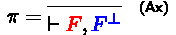
\includegraphics[width=0.95\linewidth,height=0.45\textheight,keepaspectratio]{graphic-39.pdf}\end{center}
 , one simply takes $I=F^{\perp}$, 
\begin{center}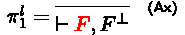
\includegraphics[width=0.95\linewidth,height=0.45\textheight,keepaspectratio]{graphic-40.pdf}\end{center}
 and 
\begin{center}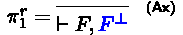
\includegraphics[width=0.95\linewidth,height=0.45\textheight,keepaspectratio]{graphic-41.pdf}\end{center}
 .\par
 
% END A1.I1.i1.p1
 
% BEGIN A1.I1.i1.p2
 
The cut between $\pi^{l}_{1}$ and $\pi^{r}_{1}$ reduces to $\pi$ by one cut-axiom reduction step.\par
 
% END A1.I1.i1.p2
 
 
\par\noindent  $\blacksquare$ 
% BEGIN A1.I1.i2.p1
 
If 
\begin{center}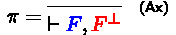
\includegraphics[width=0.95\linewidth,height=0.45\textheight,keepaspectratio]{graphic-42.pdf}\end{center}
 , the case is symmetrical taking $I=F$.\par
 
% END A1.I1.i2.p1
 
 
\par\noindent  $\blacksquare$ 
% BEGIN A1.I1.i3.p1
 
If 
\begin{center}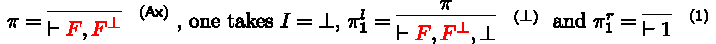
\includegraphics[width=0.95\linewidth,height=0.45\textheight,keepaspectratio]{graphic-43.pdf}\end{center}
 .\par
 
% END A1.I1.i3.p1
 
% BEGIN A1.I1.i3.p2
 
The cut of $\pi^{l}_{1}$ and $\pi^{r}_{1}$ reduces to $\pi$ by a key $1/\bot$ case.\par
 
% END A1.I1.i3.p2
 
 
\par\noindent  $\blacksquare$ 
% BEGIN A1.I1.i4.p1
 
If 
\begin{center}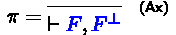
\includegraphics[width=0.95\linewidth,height=0.45\textheight,keepaspectratio]{graphic-44.pdf}\end{center}
 , the case is symmetrical to the previous one, taking $I=1$: 
\begin{center}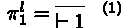
\includegraphics[width=0.95\linewidth,height=0.45\textheight,keepaspectratio]{graphic-45.pdf}\end{center}
 and 
\begin{center}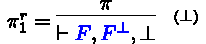
\includegraphics[width=0.95\linewidth,height=0.45\textheight,keepaspectratio]{graphic-46.pdf}\end{center}
 .\par
 
% END A1.I1.i4.p1
 
  
% END A1.SS1.p1
 
% END A1.SS1
 
% BEGIN A1.SS2
 
\par\medskip\noindent\textbf{A.2 Logical rules}\par
 
% BEGIN A1.SS2.p1
 
We analyze the possible cases for a logical rule involved in an elementary $\mathsf{PRIS}$. Note that in each case, the principal formula may be part of the left or right part of the splitting; we treat only one case each time since the other is symmetrical be taking the dual interpolant and exchanging $\pi^{L}$ and $\pi^{R}$.\par
  If the last rule is $(\mathsf{\bot})$  
% BEGIN A1.I2.ix1.p1
 
, that is if 
\begin{center}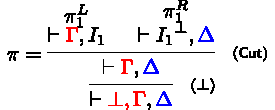
\includegraphics[width=0.95\linewidth,height=0.45\textheight,keepaspectratio]{graphic-47.pdf}\end{center}
 . By setting $I=I_{1}$, 
\begin{center}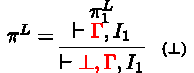
\includegraphics[width=0.95\linewidth,height=0.45\textheight,keepaspectratio]{graphic-48.pdf}\end{center}
 and $\pi^{R}=\pi^{R}_{1}$, one gets a solved $\mathsf{PRIS}$ 
\begin{center}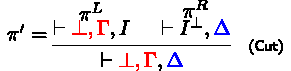
\includegraphics[width=0.95\linewidth,height=0.45\textheight,keepaspectratio]{graphic-49.pdf}\end{center}
 such that $\pi^{\prime}\longrightarrow_{\mathsf{cut}}\pi$ by a cut-commutation case.\par
 
% END A1.I2.ix1.p1
  If the last rule is $(\mathsf{1})$  
% BEGIN A1.I2.ix2.p1
 
, that is if 
\begin{center}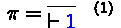
\includegraphics[width=0.95\linewidth,height=0.45\textheight,keepaspectratio]{graphic-50.pdf}\end{center}
 (which is indeed both an initial $\mathsf{PRIS}$ and an elementary $\mathsf{PRIS}$), let $I=1$ and 
\begin{center}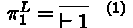
\includegraphics[width=0.95\linewidth,height=0.45\textheight,keepaspectratio]{graphic-51.pdf}\end{center}
 and 
\begin{center}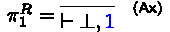
\includegraphics[width=0.95\linewidth,height=0.45\textheight,keepaspectratio]{graphic-52.pdf}\end{center}
 . One gets a solved $\mathsf{PRIS}$ $\pi^{\prime}$ such that $\pi\longleftarrow^{\star}_{\mathsf{cut}}\pi^{\prime}$ by a key $1/\bot$ case.\par
 
% END A1.I2.ix2.p1
  If the last rule is ${\text{\scriptsize$(\mathsf{\oplus^{i}})$}},i\in\{1,2\}$  
% BEGIN A1.I2.ix3.p1
 
, that is if 
\begin{center}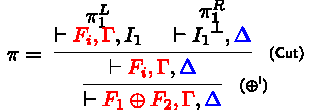
\includegraphics[width=0.95\linewidth,height=0.45\textheight,keepaspectratio]{graphic-53.pdf}\end{center}
 , then setting $I=I_{1}$, 
\begin{center}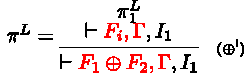
\includegraphics[width=0.95\linewidth,height=0.45\textheight,keepaspectratio]{graphic-54.pdf}\end{center}
 and $\pi^{R}=\pi_{1}^{R}$, one gets a solved $\mathsf{PRIS}$ $\pi^{\prime}$ such that $\pi\longleftarrow^{\star}_{\mathsf{cut}}\pi^{\prime}$ by a commutative reduction of $(\mathsf{Cut})$.\par
 
% END A1.I2.ix3.p1
  If the last rule is $(\mathsf{\binampersand})$  
% BEGIN A1.I2.ix4.p1
 
, that is if $\pi$ is has the following form\par
 
% END A1.I2.ix4.p1
 
% BEGIN A1.I2.ix4.p2
 
\begin{center}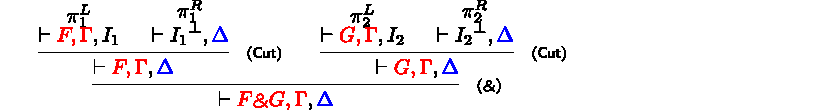
\includegraphics[width=0.95\linewidth,height=0.45\textheight,keepaspectratio]{graphic-55.pdf}\end{center}
 
% END A1.I2.ix4.p2
 
% BEGIN A1.I2.ix4.p3
 
then setting $I=I_{1}\oplus I_{2}$, 
\begin{center}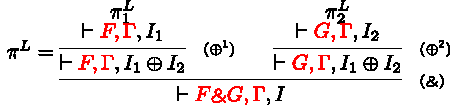
\includegraphics[width=0.95\linewidth,height=0.45\textheight,keepaspectratio]{graphic-56.pdf}\end{center}
 and 
\begin{center}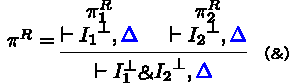
\includegraphics[width=0.95\linewidth,height=0.45\textheight,keepaspectratio]{graphic-57.pdf}\end{center}
 , one observes that\par
 
% END A1.I2.ix4.p3
 
% BEGIN A1.I2.ix4.p4
 
\begin{center}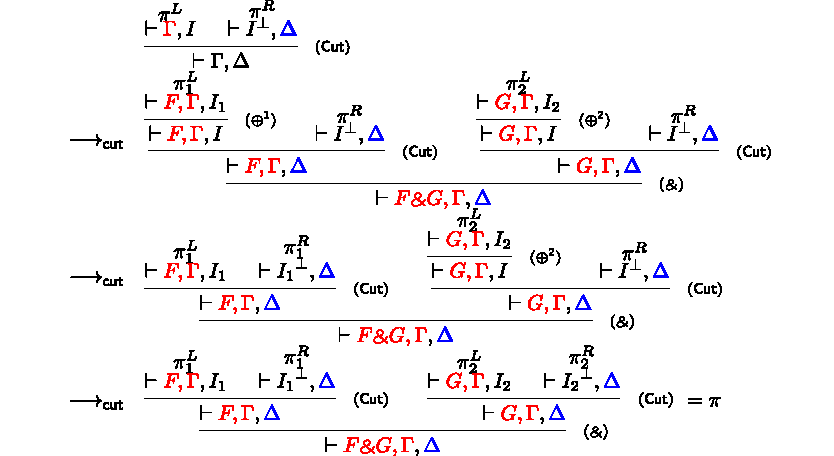
\includegraphics[width=0.95\linewidth,height=0.45\textheight,keepaspectratio]{graphic-58.pdf}\end{center}
 
% END A1.I2.ix4.p4
 
% BEGIN A1.I2.ix4.p5
 
so that $\pi$ indeed cut-expands to $\pi^{\prime}$.\par
 
% END A1.I2.ix4.p5
  If the last rule is $(\mathsf{\top})$  
% BEGIN A1.I2.ix5.p1
 
, that is if 
\begin{center}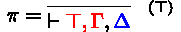
\includegraphics[width=0.95\linewidth,height=0.45\textheight,keepaspectratio]{graphic-59.pdf}\end{center}
 , by setting $I=0$, 
\begin{center}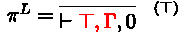
\includegraphics[width=0.95\linewidth,height=0.45\textheight,keepaspectratio]{graphic-60.pdf}\end{center}
 and 
\begin{center}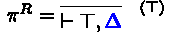
\includegraphics[width=0.95\linewidth,height=0.45\textheight,keepaspectratio]{graphic-61.pdf}\end{center}
 . Then 
\begin{center}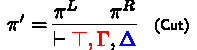
\includegraphics[width=0.95\linewidth,height=0.45\textheight,keepaspectratio]{graphic-62.pdf}\end{center}
 is a solved $\mathsf{PRIS}$ to which $\pi$ cut-expands by a $(\mathsf{\top})$ commutation case.\par
 
% END A1.I2.ix5.p1
  If the last rule is $(\mathsf{?d})$  
% BEGIN A1.I2.ix6.p1
 
, that is 
\begin{center}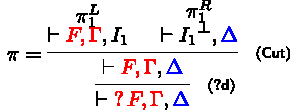
\includegraphics[width=0.95\linewidth,height=0.45\textheight,keepaspectratio]{graphic-63.pdf}\end{center}
 , then setting $I=I_{1}$, 
\begin{center}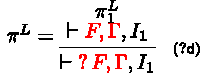
\includegraphics[width=0.95\linewidth,height=0.45\textheight,keepaspectratio]{graphic-64.pdf}\end{center}
 and $\pi^{R}=\pi^{R}_{1}$ one gets:\par
 
% END A1.I2.ix6.p1
 
% BEGIN A1.I2.ix6.p2
 
\begin{center}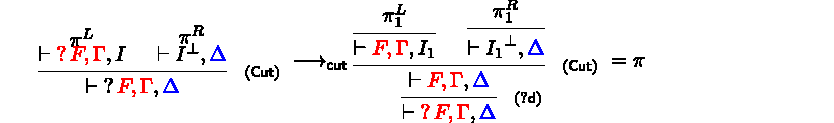
\includegraphics[width=0.95\linewidth,height=0.45\textheight,keepaspectratio]{graphic-65.pdf}\end{center}
 
% END A1.I2.ix6.p2
 
% BEGIN A1.I2.ix6.p3
 
so that $\pi$ indeed cut-expands to $\pi^{\prime}$.\par
 
% END A1.I2.ix6.p3
  If the last rule is $(\mathsf{?w})$  
% BEGIN A1.I2.ix7.p1
 
, that is 
\begin{center}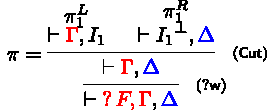
\includegraphics[width=0.95\linewidth,height=0.45\textheight,keepaspectratio]{graphic-66.pdf}\end{center}
 , then by setting $I=I_{1}$, 
\begin{center}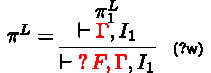
\includegraphics[width=0.95\linewidth,height=0.45\textheight,keepaspectratio]{graphic-67.pdf}\end{center}
 and $\pi^{R}=\pi^{R}_{1}$, we ensure that, since $\mathbb{V}\mathsf{oc}(I)\subseteq\mathbb{V}\mathsf{oc}(\Gamma)\cap\mathbb{V}\mathsf{oc}(\Delta)$, 
\begin{center}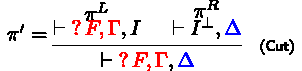
\includegraphics[width=0.95\linewidth,height=0.45\textheight,keepaspectratio]{graphic-68.pdf}\end{center}
 is indeed a solved $\mathsf{PRIS}$ and that\par
 
% END A1.I2.ix7.p1
 
% BEGIN A1.I2.ix7.p2
 
\begin{center}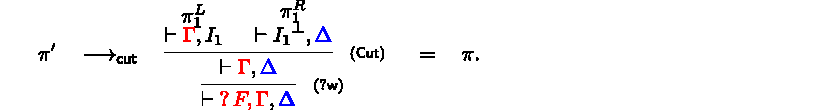
\includegraphics[width=0.95\linewidth,height=0.45\textheight,keepaspectratio]{graphic-69.pdf}\end{center}
 
% END A1.I2.ix7.p2
 
% BEGIN A1.I2.ix7.p3
 
by a cut commutation rule so that $\pi$ indeed cut-expands to $\pi^{\prime}$ as expected.\par
 
% END A1.I2.ix7.p3
  If the last rule is $(\mathsf{?c})$  
% BEGIN A1.I2.ix8.p1
 
, that is 
\begin{center}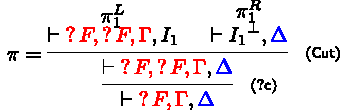
\includegraphics[width=0.95\linewidth,height=0.45\textheight,keepaspectratio]{graphic-70.pdf}\end{center}
 by setting $I=I_{1}$, 
\begin{center}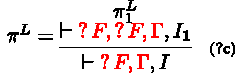
\includegraphics[width=0.95\linewidth,height=0.45\textheight,keepaspectratio]{graphic-71.pdf}\end{center}
 and $\pi^{R}=\pi^{R}_{1}$ one gets:\par
 
% END A1.I2.ix8.p1
 
% BEGIN A1.I2.ix8.p2
 
\begin{center}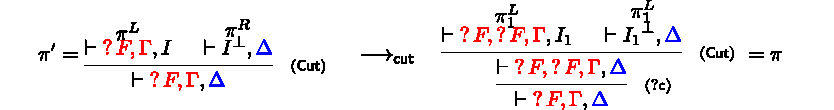
\includegraphics[width=0.95\linewidth,height=0.45\textheight,keepaspectratio]{graphic-72.pdf}\end{center}
 
% END A1.I2.ix8.p2
 
% BEGIN A1.I2.ix8.p3
 
so that $\pi^{\prime}$ is indeed a solved $\mathsf{PRIS}$ to which $\pi$ cut-expands.\par
 
% END A1.I2.ix8.p3
  If the last rule is $(\mathsf{\forall})$  
% BEGIN A1.I2.ix9.p1
 
, that is 
\begin{center}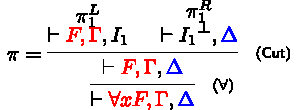
\includegraphics[width=0.95\linewidth,height=0.45\textheight,keepaspectratio]{graphic-73.pdf}\end{center}
 with $x\not\in\mathsf{FV}(\Gamma,\Delta)$ and $\mathbb{V}\mathsf{oc}(I_{1})\subseteq\mathbb{V}\mathsf{oc}(F,\Gamma)\cap\mathbb{V}\mathsf{oc}(\Delta)$. By setting $I=\exists xI_{1}$, 
\begin{center}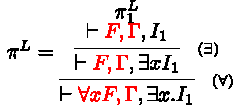
\includegraphics[width=0.95\linewidth,height=0.45\textheight,keepaspectratio]{graphic-74.pdf}\end{center}
 and 
\begin{center}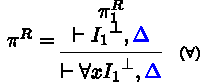
\includegraphics[width=0.95\linewidth,height=0.45\textheight,keepaspectratio]{graphic-75.pdf}\end{center}
 , one gets that: 
\begin{center}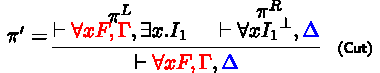
\includegraphics[width=0.95\linewidth,height=0.45\textheight,keepaspectratio]{graphic-76.pdf}\end{center}
 is a solved $\mathsf{PRIS}$ to which $\pi$ cut-expands: 
\begin{center}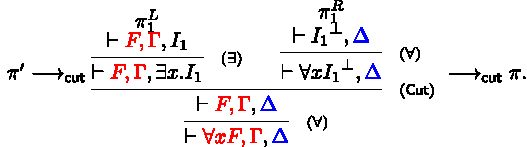
\includegraphics[width=0.95\linewidth,height=0.45\textheight,keepaspectratio]{graphic-77.pdf}\end{center}\par
 
% END A1.I2.ix9.p1
   
% END A1.SS2.p1
 
% BEGIN A1.SS2.p2
 
\par
 
% END A1.SS2.p2
 
% END A1.SS2
 
% END A1

\begin{thebibliography}{99}
\bibitem{bib-bib1} 
\par\noindent    Bahareh Afshari and Graham E. Leigh.  Lyndon interpolation for modal $\mu$-calculus.  In Aybüke Özgün and Yulia Zinova, editors, Language, Logic, and Computation - 13th International Tbilisi Symposium, TbiLLC 2019, Batumi, Georgia, September 16-20, 2019, Revised Selected Papers, volume 13206 of Lecture Notes in Computer Science, pages 197–213. Springer, 2019.  doi:10.1007/978-3-030-98479-3\_10.  

\bibitem{bib-bib2} 
\par\noindent    Michele Basaldella and Kazushige Terui.  Infinitary completeness in ludics.  In Proceedings of the 25th Annual IEEE Symposium on Logic in Computer Science, LICS 2010, 11-14 July 2010, Edinburgh, United Kingdom, pages 294–303. IEEE Computer Society, 2010.  doi:10.1109/LICS.2010.47.  

\bibitem{bib-bib3} 
\par\noindent    Michele Basaldella and Kazushige Terui.  On the meaning of logical completeness.  Log. Methods Comput. Sci., 6(4), 2010.  doi:10.2168/LMCS-6(4:11)2010.  

\bibitem{bib-bib4} 
\par\noindent    Evert W Beth.  On padoa’s method in the theory of definition.  Indagationes Mathematicae, 15:330–339, 1953.  

\bibitem{bib-bib5} 
\par\noindent    James Brotherston and Rajeev Goré.  Craig interpolation in displayable logics.  In TABLEAUX, volume 6793 of Lecture Notes in Computer Science, pages 88–103. Springer, 2011.  doi:10.1007/978-3-642-22119-4\_9.  

\bibitem{bib-bib6} 
\par\noindent    Alessandra Carbone.  Interpolants, cut elimination and flow graphs for the propositional calculus.  Ann. Pure Appl. Log., 83(3):249–299, 1997.  doi:10.1016/S0168-0072(96)00019-X.  

\bibitem{bib-bib7} 
\par\noindent    William Craig.  Linear reasoning. A new form of the Herbrand-Gentzen theorem.  J. Symb. Log., 22(3):250–268, 1957.  doi:10.2307/2963593.  

\bibitem{bib-bib8} 
\par\noindent    William Craig.  Three uses of the herbrand-gentzen theorem in relating model theory and proof theory.  J. Symb. Log., 22(3):269–285, 1957.  doi:10.2307/2963594.  

\bibitem{bib-bib9} 
\par\noindent    Djordje Cubric.  Results in categorical proof theory.  PhD thesis, McGill University, 1993.  

\bibitem{bib-bib10} 
\par\noindent    Djordje Cubric.  Interpolation property for bicartesian closed categories.  Arch. Math. Log., 33(4):291–319, 1994.  doi:10.1007/BF01270628.  

\bibitem{bib-bib11} 
\par\noindent    Pierre-Louis Curien and Hugo Herbelin.  The duality of computation.  In Martin Odersky and Philip Wadler, editors, Proceedings of the Fifth ACM SIGPLAN International Conference on Functional Programming (ICFP ’00), Montreal, Canada, September 18-21, 2000, pages 233–243. ACM, 2000.  doi:10.1145/351240.351262.  

\bibitem{bib-bib12} 
\par\noindent    Pierre-Louis Curien and Guillaume Munch-Maccagnoni.  The duality of computation under focus.  In Cristian S. Calude and Vladimiro Sassone, editors, Theoretical Computer Science - 6th IFIP TC 1/WG 2.2 International Conference, TCS 2010, Held as Part of WCC 2010, Brisbane, Australia, September 20-23, 2010. Proceedings, volume 323 of IFIP Advances in Information and Communication Technology, pages 165–181. Springer, 2010.  doi:10.1007/978-3-642-15240-5\_13.  

\bibitem{bib-bib13} 
\par\noindent    Vincent Danos, Jean-Baptiste Joinet, and Harold Schellinx.  A new deconstructive logic: Linear logic.  J. Symb. Log., 62(3):755–807, 1997.  doi:10.2307/2275572.  

\bibitem{bib-bib14} 
\par\noindent    Jeremy E. Dawson, James Brotherston, and Rajeev Goré.  Machine-checked interpolation theorems for substructural logics using display calculi.  In IJCAR, volume 9706 of Lecture Notes in Computer Science, pages 452–468. Springer, 2016.  doi:10.1007/978-3-319-40229-1\_31.  

\bibitem{bib-bib15} 
\par\noindent    Adrien Deloro.  Cours de logique mathématique.  Draft of a book on mathematical logic, 2025.  URL: https://webusers.imj-prg.fr/˜adrien.deloro/index.php?topic=teaching\&page=logique.  

\bibitem{bib-bib16} 
\par\noindent    Kosta Došen.  Logical Consequence: A Turn in Style, pages 289–311.  Springer Netherlands, Dordrecht, 1997.  doi:10.1007/978-94-017-0487-8\_15.  

\bibitem{bib-bib17} 
\par\noindent    Solomon Feferman.  Harmonious logic: Craig’s interpolation theorem and its descendants.  Synthèse, 164(3):341–357, 2008.  doi:10.1007/S11229-008-9354-2.  

\bibitem{bib-bib18} 
\par\noindent    Melvin Fitting.  Linear reasoning in modal logic.  J. Symb. Log., 49(4):1363–1378, 1984.  doi:10.2307/2274285.  

\bibitem{bib-bib19} 
\par\noindent    Jean-Yves Girard.  Linear logic.  Theoretical Computer Science, 50(1):1–101, 1987.  doi:10.1016/0304-3975(87)90045-4.  

\bibitem{bib-bib20} 
\par\noindent    Jean-Yves Girard.  Proof theory and logical complexity.  Bibliopolis, 1987.  

\bibitem{bib-bib21} 
\par\noindent    Thomas A. Henzinger, Ranjit Jhala, Rupak Majumdar, and Kenneth L. McMillan.  Abstractions from proofs.  SIGPLAN Not., 39(1):232–244, January 2004.  doi:10.1145/982962.964021.  

\bibitem{bib-bib22} 
\par\noindent    Stefan Hetzl and Raheleh Jalali.  On the completeness of interpolation algorithms.  In Pawel Sobocinski, Ugo Dal Lago, and Javier Esparza, editors, Proceedings of the 39th Annual ACM/IEEE Symposium on Logic in Computer Science, LICS 2024, Tallinn, Estonia, July 8-11, 2024, pages 45:1–45:13. ACM, 2024.  doi:10.1145/3661814.3662112.  

\bibitem{bib-bib23} 
\par\noindent    Makoto Kanazawa.  Computing interpolants in implicational logics.  Annals of Pure and Applied Logic, 142(1):125–201, 2006.  doi:10.1016/j.apal.2005.12.014.  

\bibitem{bib-bib24} 
\par\noindent    Roman Kuznets.  Multicomponent proof-theoretic method for proving interpolation properties.  Ann. Pure Appl. Log., 169(12):1369–1418, 2018.  doi:10.1016/J.APAL.2018.08.007.  

\bibitem{bib-bib25} 
\par\noindent    Shoji Maehara.  On the interpolation theorem of Craig.  Sûgaku, 12(4), 1960.  

\bibitem{bib-bib26} 
\par\noindent    Ralph Matthes.  Interpolation for natural deduction with generalized eliminations.  In Reinhard Kahle, Peter Schroeder-Heister, and Robert Stärk, editors, Proof Theory in Computer Science, pages 153–169, Berlin, Heidelberg, 2001. Springer Berlin Heidelberg.  doi:10.1007/3-540-45504-3\_10.  

\bibitem{bib-bib27} 
\par\noindent    Kenneth L. McMillan.  Interpolation and model checking.  In Edmund M. Clarke, Thomas A. Henzinger, Helmut Veith, and Roderick Bloem, editors, Handbook of Model Checking., pages 421–446. Springer, 2018.  doi:10.1007/978-3-319-10575-8\_14.  

\bibitem{bib-bib28} 
\par\noindent    Grigori Mints.  Finite investigations of transfinite derivations.  Journal of Soviet Mathematics, 10:548–596, 1978.  

\bibitem{bib-bib29} 
\par\noindent    Guillaume Munch-Maccagnoni.  Focalisation and Classical Realisability.  In Erich Grädel and Reinhard Kahle, editors, Computer Science Logic ’09, volume 5771 of Lecture Notes in Computer Science, pages 409–423. Springer, Heidelberg, 2009.  doi:10.1007/978-3-642-04027-6\_30.  

\bibitem{bib-bib30} 
\par\noindent    Guillaume Munch-Maccagnoni.  Syntax and Models of a non-Associative Composition of Programs and Proofs.  PhD thesis, Univ. Paris Diderot, 2013.  

\bibitem{bib-bib31} 
\par\noindent    Dag Prawitz.  Natural Deduction: A Proof-Theoretical Study.  Dover Publications, Mineola, N.Y., 1965.  

\bibitem{bib-bib32} 
\par\noindent    João Rasga, Walter Alexandre Carnielli, and Cristina Sernadas.  Interpolation via translations.  Math. Log. Q., 55(5):515–534, 2009.  doi:10.1002/MALQ.200810013.  

\bibitem{bib-bib33} 
\par\noindent    A. Robinson.  A result of consistency and its application to the theory of definition.  Indagationes Mathematicae, 18, 1956.  

\bibitem{bib-bib34} 
\par\noindent    Dirk Roorda.  Interpolation in fragments of classical linear logic.  The Journal of Symbolic Logic, 59(2):419–444, 1994.  doi:10.2307/2275398.  

\bibitem{bib-bib35} 
\par\noindent    Kurt Schütte.  Proof theory, volume 85.  Springer, 1977.  

\bibitem{bib-bib36} 
\par\noindent    D. S. Shamkanov.  Circular proofs for the Gödel-Löb provability logic.  Mathematical Notes, 96(3), 2014.  doi:10.1134/S0001434614090326.  

\bibitem{bib-bib37} 
\par\noindent    Lutz Strassburger.  Linear Logic and noncommutativity in the Calculus of Structures.  PhD thesis, TU Dresden, 2003.  

\bibitem{bib-bib38} 
\par\noindent    Amirhossein Akbar Tabatabai and Raheleh Jalali.  Universal proof theory: Semi-analytic rules and craig interpolation.  Ann. Pure Appl. Log., 176(1):103509, 2025.  doi:10.1016/J.APAL.2024.103509.  

\bibitem{bib-bib39} 
\par\noindent    Gaisi Takeuti.  Proof theory, volume 81.  Courier Corporation, 2013.  

\bibitem{bib-bib40} 
\par\noindent    A. S. Troelstra and H. Schwichtenberg.  Basic Proof Theory.  Cambridge Tracts in Theoretical Computer Science. Cambridge University Press, 2 edition, 2000.  

\end{thebibliography}
\end{document}
